\documentclass[natbib,preprint]{sigplanconf}

\usepackage[usenames]{color}
\definecolor{citationcolour}{rgb}{0,0.4,0.2}
\definecolor{linkcolour}{rgb}{0,0,0.8}
\usepackage{hyperref}
\hypersetup{colorlinks=true,
            urlcolor=linkcolour,
            linkcolor=linkcolour,
            citecolor=citationcolour,
            pdftitle=Relational Parametricity for Algebraically-Indexed Types,
            pdfauthor={Robert Atkey, Neil Ghani, Patricia Johann, Andrew Kennedy},
            pdfkeywords={}}  
\def\sectionautorefname{Section}
\def\subsectionautorefname{Section}

\title{Relational Parametricity for Algebraically Indexed Types}

\authorinfo{Robert Atkey\and Neil Ghani\\\and Patricia Johann}
           {University of Strathclyde}
           {\{Robert.Atkey,Neil.Ghani,Patricia.Johann\}@cis.strath.ac.uk}

\authorinfo{Andrew Kennedy}
           {Microsoft Research}
           {}

\usepackage{mathpartir}
\usepackage{amsmath}
\usepackage{amssymb}
\usepackage{amsthm}
\usepackage{stmaryrd}
\usepackage[all]{xy}

\newcommand{\GA}{\mathrm{GA}}
\newcommand{\GL}{\mathrm{GL}}
\newcommand{\Is}{\mathrm{Is}}
\newcommand{\Orth}{\mathrm{O}}
\newcommand{\SOrth}{\mathrm{SO}}
\newcommand{\Transl}{\mathrm{T}}
\newcommand{\Scale}{\mathrm{Scale}}


\newcommand{\sepbar}{\mathrel|}

\newcommand{\Rel}{\mathrm{Rel}}
\newcommand{\relArrow}{\mathrel{\widehat\to}}
\newcommand{\relTimes}{\mathrel{\widehat\times}}
\newcommand{\relSum}{\mathrel{\widehat+}}

\newcommand{\setOfIntegers}{\mathbb{Z}}
\newcommand{\setOfBooleans}{\{\tmTT, \tmFF\}}

\newcommand{\id}{\mathrm{id}}

\newcommand{\SortSet}{\mathit{Sort}}
\newcommand{\IndexOpSet}{\mathit{IndexOp}}
\newcommand{\PrimTypeSet}{\mathit{PrimType}}
\newcommand{\IndexAxiomSet}{\mathit{IndexAx}}

\newcommand{\indexOp}[1]{\texttt{#1}}
\newcommand{\idxTms}[2]{\mathrm{IdxTm}(#1 \vdash #2)}
\newcommand{\idxTmAS}[1]{\mathrm{IdxTm}(#1)}

\newcommand{\tyInt}{\texttt{int}}
\newcommand{\tyBool}{\texttt{bool}}
\newcommand{\tyUnit}{\texttt{unit}}
\newcommand{\tyPrim}[2]{\texttt{#1}\langle #2 \rangle}
\newcommand{\tyPrimNm}[1]{\texttt{#1}}
\newcommand{\primTyArity}{\mathrm{tyArity}}
\newcommand{\indexOpArity}{\mathrm{opArity}}

\newcommand{\tyArr}{\to}
\newcommand{\tyProduct}{\times}
\newcommand{\tyX}[1]{\texttt{X}\langle #1 \rangle}
\newcommand{\isType}{\textsf{ type}}
\newcommand{\isCtxt}{\textsf{ ctxt}}
\newcommand{\Ty}{\textsf{Ty}}
\newcommand{\ty}{\textsf{ty}}
\newcommand{\subst}[2]{\mathrm{Subst}(#1,#2)}

\newcommand{\tmTT}{\texttt{tt}}
\newcommand{\tmFF}{\texttt{ff}}

\newcommand{\relEnv}[1]{\mathcal{#1}}
\newcommand{\tySem}[1]{\llbracket #1 \rrbracket^{\mathcal{T}}}
\newcommand{\ctxtSem}[1]{\llbracket #1 \rrbracket^{\mathcal{C}}}
\newcommand{\tmSem}[1]{\llbracket #1 \rrbracket^{\mathit{tm}}}
\newcommand{\tyPrimSem}[1]{\llbracket #1 \rrbracket^{\mathcal{T}_0}}
\newcommand{\rsem}[3]{\llbracket #1 \rrbracket^{\mathcal{R}}_{#2}{#3}}
\newcommand{\extends}[2]{\mathsf{ext}(#1,#2)}

\newtheorem{lemma}{Lemma}
\newtheorem{theorem}{Theorem}
\newtheorem{example}{Example}
\newcommand{\lemref}[1]{\hyperref[#1]{Lemma \ref*{#1}}}
\newcommand{\thmref}[1]{\hyperref[#1]{Theorem \ref*{#1}}}
\newcommand{\propref}[1]{\hyperref[#1]{Proposition \ref*{#1}}}
\newcommand{\corref}[1]{\hyperref[#1]{Corollary \ref*{#1}}}
\newcommand{\conref}[1]{\hyperref[#1]{Conjecture \ref*{#1}}}
\newcommand{\exref}[1]{\hyperref[#1]{Example \ref*{#1}}}
\newcommand{\statementref}[1]{\hyperref[#1]{Statement \ref*{#1}}}

\newcommand{\sem}[1]{\llbracket #1 \rrbracket}
\newcommand{\isDefinedAs}{\stackrel{\mathit{def}}=}

\begin{document}

\maketitle

\begin{abstract}
  
\end{abstract}

\category{D.1.1}{Programming techniques}{Applicative (functional)
  programming} \category{D.2.4}{Software Engineering}{Software/Program
  Verification} \category{D.3.3}{Programming Languages}{Language
  Constructs and Features---Data types and structures}

\terms
  Languages, Theory, Types

\keywords
  parametricity, dimension types, computational geometry

%%%%%%%%%%%%%%%%%%%%%%%%%%%%%%%%%%%%%%%%%%%%%%%%%%%%%%%%%%%%%%%%%%%%%%%%%%%%%%
%%%%%%%%%%%%%%%%%%%%%%%%%%%%%%%%%%%%%%%%%%%%%%%%%%%%%%%%%%%%%%%%%%%%%%%%%%%%%%
\section{Introduction}
\label{sec:introduction}
The best way we know of describing the semantics of parametric
polymorphism is \emph{relational parametricity}, whose central result
is Reynolds' Abstraction Theorem~\cite{reynolds83types}. Its striking
consequences include the well-known ``free theorems'' for polymorphic
types~\cite{wadler89theorems}, non-inhabitation results, and precise
correspondences between System F encodings and algebraic
datatypes~\cite{PittsAM:parpoe}, abstract data types, and, most
recently, higher-order encodings of binder
syntax~\cite{syntaxforfree}.

Relational parametricity is in essence a principle of
\emph{invariance}: the behaviour of polymorphic code is invariant
under changes of data representation. For example, the type
$\forall\alpha.\tyPrim{list}\alpha\to\tyPrim{list}\alpha$
tells us that any transformation applied to elements of
the input list will be reflected by the same transformation applied
to elements of the result. 
Invariance results also abound in
mathematics and physics. The area of a triangle is invariant with
respect to isometries of the Euclidean plane; the determinant of a
matrix is invariant under changes of basis; and Newton's laws are the
same in all inertial frames. Typically, the 
transformations under which invariants are preserved have interesting structure: 
for example, translations in
the Euclidean plane form an abelian group.

Inspired by this connection, we study type systems that
capture rich invariants through types indexed by attributes with
algebraic structure.  For example, in computational geometry, points
in the plane can be indexed by attributes representing affine
transformations; in information-flow security, computations can be
indexed by principals; in differential privacy, types can be indexed
by `distance'. Types that are polymorphic over such indices induce
invariance properties and abstraction barriers beyond those introduced
by their unindexed versions, as we shall illustrate.  This generalises
previous work by the third author on types parameterized by
units of measure, whose invariance properties relate to changes of
units, or \emph{scaling}~\cite{kennedy97relational}.

Our motivations for studying algebraically indexed types are
threefold. First, we believe that, as with
units of measure~\cite{fsharp}, practical programming language
extensions will follow. For example, in computational geometry and
graphics, attributes on points, vectors, and other geometric types
could be used to prevent the mixing of different coordinate systems,
or `frames'. Second, type-based static analyses can be based on
indexed types, for example, in effect systems~\cite{benton06reading},
and, more speculatively, in continuity
analysis~\cite{chaudhuri10continuity}.  Finally, we believe that
expressing algebraic invariants through types has the potential to
offer slick proof techniques for mechanized
mathematics. Harrison has applied the
invariance properties of geometric primitives to create elegant proofs
in geometry, based on `without loss of
generality' principles~\cite{harrison09without}. The invariance properties are expressed 
and propagated using ad-hoc tactics; our types offer a more principled
means of achieving the same end, and the `wlog' principle itself
is expressed through type isomorphisms.

We follow the mantra \emph{semantics first, syntax later} in studying
types with algebraic structure. We have not yet built a practical
programming language that supports algebraically indexed types; nor
have we designed type checking, type inference, or static analysis
algorithms.  But when we do so, the semantics will guide us. The fact
that zero is polymorphic in units of measure (it can be given type $\forall
u.\tyPrim{real}u$) whereas other constants are dimensionless (having
type $\tyPrim{real}1$) is justified by the invariance properties
induced by the types: zero is invariant under scaling, other constants
are not. For less trivial constants and operations, the appropriate types are
not so apparent, as we shall see, but invariance properties expressed by
the semantics guide us in assigning appropriate types. Semantics does not lie!


\paragraph{Invariance}
To illustrate type-induced invariance properties, consider
2-dimensional geometry. 
A function $\mathit{areaTri}$ that computes the area of a triangle
can be assigned the type:
$\tyPrimNm{vec}\times\tyPrimNm{vec}\times\tyPrimNm{vec}\tyArr\tyReal$.
But we can also assign it the following more expressive polymorphic
type:
\[
\mathrm{areaTri} : \forall t\mathord:\SynTransl{2}.
  \tyPrim{vec}{t} \times \tyPrim{vec}{t} \times \tyPrim{vec}{t} \to \tyReal \\
\]
This type expresses the fact that if each of the arguments to $\mathrm{areaTri}$
is translated by the same vector, then the result remains the same,
that is, it is \emph{invariant} under translation. Formally, for any 
vector $\vec t$,
\[
\mathrm{areaTri}\;(\vec{t} + \vec{v_1}, \vec{t} + \vec{v_2}, \vec{t} + \vec{v_3}) = 
\mathrm{areaTri}\;(\vec{v_1}, \vec{v_2}, \vec{v_3})
\]

Transformations typically \emph{compose} in various
ways, and the compositions satisfy algebraic laws. For example, 
we can assign a function that computes the area of a circle given its
radius the following polymorphic type:
\[
\mathrm{areaCircle} : \forall s\mathord:\SynGL{1}.\tyPrim{real}{s}\to
\tyPrim{real}{s\cdot s}
\]
This captures the fact that the area of a circle varies as the square
of its radius, i.e., $\mathrm{areaCircle}(k r) = k^2\cdot
\mathrm{areaCircle}(r)$ for any $k\neq 0$ (the `sorts' $\SynTransl{2}$ and
$\SynGL{1}$ will be explained later).  Here, $s$ 
can be interpreted as the \emph{units of measure} of the argument to
$\mathrm{areaCircle}$, and `$\cdot$' composes units using the
product. We can also add an inverse operation and identity unit of
measure $1$, and then impose the algebraic laws of abelian
groups. This permits identification of, for example,
$\tyPrim{real}{s\cdot s^{-1}}$ with the type
$\tyPrim{real}{1}$ of dimensionless constants.

\paragraph{Abstraction}
In his original paper on parametricity, Reynolds asserted that
\emph{type structure is a syntactic discipline for enforcing levels of
  abstraction}.  We see something analogous here: if all primitive
operations are given types that reflect their behaviour under
translation, then there is no way to `break' this property. For
example, there is no way that $\mathrm{areaTri}$ can depend on the
actual coordinates of its inputs. Furthermore, the distinction between
points and vectors that is often enforced through abstract data
types~\cite{CGAL} is captured here by indices instead. For example,
the operation that takes two points and computes their vector
difference can be assigned the type
$\forall t\mathord:\SynTransl{2}.\tyPrim{vec}t\times\tyPrim{vec}t\to\tyPrim{vec}0$,
reflecting the invariance of the result (a pure vector) under
translations of the point arguments. As a result through types alone
we can, in essence, derive so-called \emph{coordinate-free}
geometry~\cite{CFGADT}.

The invariance properties discussed above can be seen as ``free
theorems''~\cite{wadler89theorems}, but the abstraction afforded by
polymorphic indexed types can also induce interesting type
\emph{isomorphisms}.  The type of $\mathrm{areaCircle}$ above is in
fact isomorphic to $\tyPrim{real}{1}$. A moment's thought reveals why:
what possible unary functions can be constructed whose outputs scale
as the square of the scaling of their inputs?  Answer: just those
functions of the form~$\lambda x. k x^2$ for some constant~$k$.  In
this case, of course, we expect that~$k = \pi$.

\paragraph{Relational parametricity}
To derive such invariance and abstraction properties of types, we
adopt the techniques of relational parametricity. Over an underlying
index-erasure semantics we construct binary relations parameterised by
an environment $\rho$ that describes how values of primitive type are
related according to their indices.  For example, values $v$ and $w$
of type $\tyPrim{real}s$ are related when $v$ ``scales to'' $w$
according to an interpretation of $s$ (i.e., $w=\rho(s)\cdot
v$).  Values of polymorphic type are related exactly when they are
related for all possible interpretations of the quantified
variable. For example, values $v$ and $w$ of type
$\forall t\mathord:\SynTransl{2}.\tyPrim{vec} t\to
\tyPrim{vec} t$ are related when they are related at type
$\tyPrim{vec} t\to\tyPrim{vec}t$ for all translations
$\vec t\in\Transl{2}$ associated with $t$.

As it happens, the relational interpretations given above are
functional, relating one value uniquely to another. Other applications
make use of primitive relations that are not simple functions.
For example, in a type system in which the index in
$\tyPrim{real}s$ is interpreted not as a unit of measure, but as
a measure of \emph{closeness}, two values $x$ and $y$ of this type are
related if $|x-y| < \rho(s)$ for a positive real number
$\rho(s)$.  Rather beautifully, the standard notion of uniform
continuity can then be expressed as %a type:
%\begin{displaymath}
 $ \forall \epsilon \mathord: \mathsf{R}^{>0}.\ \exists \delta\mathord: \mathsf{R}^{>0}.\ \tyPrim{real}{\delta} \to \tyPrim{real}{\epsilon}$.
%\end{displaymath}


% Possible angles of attack:
% \begin{itemize}
% \item Parametric polymorphic types allow us to prevent
%   over-specification of the behaviour of programs. For instance, the
%   type $\forall \alpha. [\alpha] \to [\alpha]$ is a generalisation of
%   the types $[\mathsf{int}] \to [\mathsf{int}]$ and $[\mathsf{char}]
%   \to [\mathsf{char}]$. Either of the latter two types over-specify
%   the behaviour of the function.
% \item There are other cases of programs that are over-specified. The
%   leading example we just below is of geometric programs that
%   manipulate coordinate data. Often, programs that manipulate
%   coordinate data are insensitive to geometric transformations. For
%   example, a program that computes the area of a triangle described by
%   three points is insensitive to translations or rotations applied to
%   all three points.
% \item 
% \end{itemize}

% There are three main points to get across:
% \begin{enumerate}
% \item Why algebraically indexed types?
% \item Why relational parametricity?
% \item Why study them together?
% \end{enumerate}

\subsection{Contributions}
\label{sec:contributions}

\begin{figure}
  \centering
  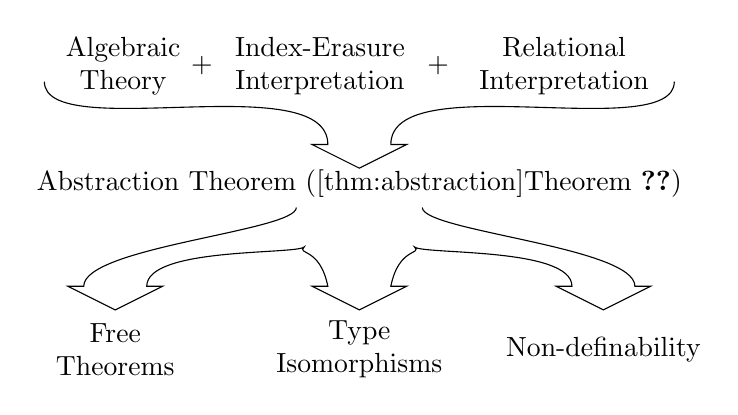
\begin{tikzpicture}
  \node at (-3,0.8) [rectangle,style={align=center}] {Algebraic \\ Theory};
  \node at (-2,0.8) {$+$};
  \node at (-0.5,0.8) [rectangle,style={align=center}] {Index-Erasure \\ Interpretation};
  \node at (1,0.8) {$+$};
  \node at (2.6,0.8) [rectangle,style={align=center}] {Relational \\ Interpretation};
  
  \draw plot (-4,0.6) .. controls (-4,-0.2) and (-0.4,0.8) .. (-0.4,-0.2)
             -- (-0.6,-0.2) -- (0,-0.5) -- (0.6,-0.2) --
             (0.4,-0.2) .. controls (0.4,0.8) and (4,-0.2) .. (4,0.6);

  \node at (0,-0.7) [rectangle,style={align=center}] {Abstraction Theorem (\thmref{thm:abstraction})};

  \draw plot (-0.8,-1) .. controls (-0.8,-1.3) and (-3.5,-1.5) .. (-3.5,-2)
             -- (-3.7,-2) -- (-3.1,-2.3) -- (-2.5,-2) -- 
             (-2.7,-2) .. controls (-2.7,-1.5) and (-0.8,-1.6) .. (-0.7,-1.5)
                       .. controls (-0.8,-1.6) and (-0.5,-1.5) ..
             (-0.4,-2) -- (-0.6,-2) -- (0,-2.3) -- (0.6,-2) --
             (0.4,-2) .. controls (0.5,-1.5) and (0.8,-1.6) .. (0.7,-1.5)
                      .. controls (0.8,-1.6) and (2.7,-1.5) ..
             (2.7,-2) -- (2.5,-2) -- (3.1,-2.3) -- (3.7,-2) -- (3.5,-2)
                      .. controls (3.5,-1.5) and (0.8,-1.3) .. (0.8,-1);

  \node at (-3.1,-2.8) [rectangle,style={align=center}] {Free \\ Theorems};
  \node at (0,-2.8) [rectangle,style={align=center}] {Type \\ Isomorphisms};
  \node at (3.1,-2.8) [rectangle,style={align=center}] {Non-definability};
\end{tikzpicture}
  \caption{Summary of the Paper}
  \label{fig:summary}
\end{figure}

This paper makes the following specific contributions:
\begin{itemize}
\item 
We present a collection of compelling examples of algebraically
indexed types, including a novel type system for geometry, a
refined type system for information flow based on logic, and a simple
type system with distance-indexed types.
\item 
We formulate a type system that can either be used as a programming
language in its own right, or as the target of type-based
analyses. The type system consists of the usual type constructors
together with a collection of indexed primitive types, universal and
existential quantification over the indices, and a multi-sorted
equational theory for indices.
\item
We describe a relational semantics for the type system and prove an
analogue of Reynolds' Abstraction Theorem, for a given \emph{model}
of index sorts and relational interpretation of primitive types.
We prove that the semantics soundly approximates contextual equivalence.
\item
For each of our main examples we deduce free theorems that are
consequences of our Abstraction Theorem, prove non-definability
results, and derive interesting type isomorphisms. \autoref{fig:summary}
illustrates the central position of our analogue of Reynolds' Abstraction
Theorem (\thmref{thm:abstraction}) in these results.
\item
We improve on the earlier semantics of
units of measure~\cite{kennedy97relational} in a number of ways.  By
extending the language of units with an `absolute value' operation, we
can give more precise types and obtain more general invariance
properties.  The relational interpretation for units is both simpler
and more flexible, and we derive slicker proofs of non-definability,
and new results.  Our notion of type isomorphism is stronger than
previously, being based on contextual equivalence.
\end{itemize}
We have fully formalised our framework and most examples in Coq,
using strongly-typed term representations
throughout~\cite{TypedSyntax}. The formalisation is available from
\\{\small \url{https://github.com/bobatkey/algebraically-indexed-types}}



%%% Local Variables:
%%% TeX-master: "paper"
%%% End:

\section{Motivating Examples}
\label{sec:motivating-examples}

In this section we present three motivating examples that illustrate
why algebraically indexed types are an interesting object of study,
and why relational semantics is a useful and powerful way of studying
the semantics of algebraically indexed types. The common theme running
through each of the examples we present in this section is the use of
algebraic indexing to capture the invariance \emph{and} variance of
programs with respect to changes in their environment. The first
example that we consider is Kennedy's original units of measure
system.

\subsection{Units of Measure and Scale Invariance}
\label{sec:units-of-measure-example-intro}

FIXME:
\begin{enumerate}
\item Describe the units of measure system
\item Describe the concept of scale invariance
\item Describe the consequences of scale invariance
\end{enumerate}

\subsection{Vector Spaces and Frame Invariance}
\label{sec:vector-spaces-intro}

FIXME: integrate a cut-down version of the geometry-invariance note
here.

\subsection{Security Types and Satisfaction Invariance}
\label{sec:security-types-intro}

FIXME: re-do the security types example from the previous draft, but
making sure to re-phrase everything in terms of ``satisfaction''.

\subsection{Taking Stock}
\label{sec:taking-stock}

Main points to get across:
\begin{enumerate}
\item Algebraic indexing captures both the invariance properties as
  well as the variance properties of the action of programs.
\item Relational semantics provides a powerful way to connect the
  invariance and variance properties to types.
\item The assignment of relational semantics to algebraic indexed may
  not necessarily be compositional.
\end{enumerate}


%%% Local Variables:
%%% TeX-master: "paper"
%%% End:

\section{Background and Related Work}
\label{sec:background}

\begin{enumerate}
\item Reynolds \cite{reynolds83types}
\item Kennedy \cite{kennedy97relational}
\item Gallier (for information on geometry) \cite{gallier11geometric}
\item Tse and Zdancewic, and Sabelfeld and Sands, for information flow \cite{sabelfeld01per}
\item Chaudhuri, Gulwani and Lublinerman, for continuity analysis \cite{chaudhuri10continuity}
\end{enumerate}

We discuss further related work in \autoref{sec:discussion}.

%%% Local Variables:
%%% TeX-master: "paper"
%%% End:

\section{A General Framework}
\label{sec:a-general-framework}

%In this section 
We now present our framework for algebraically
indexed types. % and representation independence. %We define the syntax
%and semantics of algebraically indexed types, then their semantics
%and finally we present a general programming language for
%algebraically indexed types, together with an abstraction theorem.

\subsection{Algebraically-Indexed Types}
\label{sec:algebraically-indexed-types}

The index expressions and types of an instantiation of our general
framework are derived from the following data:
\begin{enumerate}
\item A collection $\SortSet$ of index sorts. We use the
  meta-syntactic variables $s,s_1,s_2,...$ for arbitrary sorts taken
  from $\SortSet$.
\item A collection $\IndexOpSet$ of index operations, with a function
  $\indexOpArity : \IndexOpSet \to \SortSet^* \times \SortSet$. (We use
  the notation $A^*$ to denote the set of lists of elements of some
  set $A$.)
\item A collection $\PrimTypeSet$ of primitive types, with a function
  $\primTyArity : \PrimTypeSet \to \SortSet^*$. %, describing the sorts
%  of the arguments of each primitive type.
\end{enumerate}

\begin{example}[Two-Dimensional Geometry]
  \label{ex:two-dim-geo-operations}
  The two-dimensional geometry system has a sort for each of the
  geometric groups mentioned in \autoref{sec:motivating-examples}, so
  $\SortSet = \{\SynTransl{2}, \SynGL{2}, \SynOrth{2}, \SynGL{1} \}$.
  %For the index operations, 
  We have additive group structure on $\SynTransl{2}$, multiplicative
  group structure on $\SynGL{1}$, $\SynGL{2}$, and $\SynOrth{2}$,
  injections from $\SynOrth{2}$ and $\SynGL{1}$ into $\SynGL{2}$,
  determinant, and absolute value. Thus, $\IndexOpSet = \{ 0, +, -,
  1_G, -\cdot_G-, -^{-1_G}, \iota_O, \iota_1, \det, |\cdot| \}$, where
  $G \in \{\SynGL{1}, \SynGL{2}, \SynOrth{2}\}$, and
  %  with the following assignment of arities:
  \begin{displaymath}
    \begin{array}{@{}l@{\hspace{0em}=\hspace{0em}}l@{\hspace{0.5em}}l@{\hspace{0em}=\hspace{0em}}l}
      \indexOpArity(0) & ([], \SynTransl{2}) &
      \indexOpArity(1_G) & ([], G) \\
      \indexOpArity(+) & ([\SynTransl{2}, \SynTransl{2}], \SynTransl{2}) &
      \indexOpArity(\cdot_G) & ([G,G],G) \\
      \indexOpArity(-) & ([\SynTransl{2}], \SynTransl{2}) &
      \indexOpArity(^{-1_G}) & ([G], G) \\
      \indexOpArity(\iota_o) & ([\SynOrth{2}], \SynGL{2}) &
      \indexOpArity(\iota_1) & ([\SynGL{1}], \SynGL{2}) \\
      \indexOpArity(\det) & ([\SynGL{2}], \SynGL{1}) &
      \indexOpArity(|\cdot|) & ([\SynGL{1}], \SynGL{1})
    \end{array}
  \end{displaymath}
%  The intended interpretations of the top three pairs of operations
%  are group unit, group combination and group negation,
%  respectively. 
%  When we discuss equational theories on index expressions 
%in \autoref{sec:type-equality} 
%we will impose the (abelian) group laws. For this example, 
We also have $\PrimTypeSet = \{ \tyPrimNm{vec},
  \tyPrimNm{real} \}$, with $\primTyArity(\tyPrimNm{vec}) =
           [\SynGL{2}, \SynTransl{2}]$ and
           $\primTyArity(\tyPrimNm{real}) = [\SynGL{1}]$.
\end{example}

We assume a countably infinite collection of index variable names $i,
i_1, i_2,\ldots$. \emph{Index contexts} $\Delta = i_1 \mathord: s_1,
..., i_n \mathord: s_n$ are lists of variable/sort pairs such that
all the variable names are distinct.
\begin{figure*}[t]
  \centering
  % \textbf{Index contexts}\\

  % $\Delta = i_1 \mathord: s_1, ..., i_n \mathord: s_n$, where each $s_i \in \SortSet$ and no variable name is repeated.

  % \bigskip

  {\small
  \textbf{Well-sorted index expressions}
  \begin{mathpar}
    \inferrule* [right=IVar]
    {i : s \in \Delta}
    {\Delta \vdash i : s}
    
    \inferrule* [right=IOp]
    {\indexOp{f} \in \mathit{IndexOp} \\
      \indexOpArity(\indexOp{f}) = ([s_1,...,s_n], s) \\
      \{\Delta \vdash e_j : s_j\}_{1 \leq j \leq n}}
    {\Delta \vdash \indexOp{f}(e_1, ..., e_n) : s}
  \end{mathpar}

  \bigskip

  \textbf{Well-indexed types}
  \begin{mathpar}
    \inferrule* [right=TyPrim]
    {\tyPrimNm{X} \in \mathit{PrimType} \\\\
      \primTyArity(\tyPrimNm{X}) = [s_1,...,s_n] \\
      \{\Delta \vdash e_j : s_j\}_{1\leq j \leq n}}
    {\Delta \vdash \tyPrim{X}{e_1,...,e_n} \isType}

    \inferrule* [right=TyUnit]
    { }
    {\Delta \vdash \tyUnit \isType}

    \inferrule* [right=TyArr]
    {\Delta \vdash A \isType \\ \Delta \vdash B \isType}
    {\Delta \vdash A \tyArr B \isType}

    \inferrule* [right=TyTuple]
    {\Delta \vdash A \isType \\ \Delta \vdash B \isType}
    {\Delta \vdash A \tyProduct B \isType}

    \inferrule* [right=TySum]
    {\Delta \vdash A \isType \\ \Delta \vdash B \isType}
    {\Delta \vdash A + B \isType}
    
    \inferrule* [right=TyForall] %FIXME: macroize forall
    {\Delta, i \mathord: s \vdash A \isType}
    {\Delta \vdash \forall i \mathord: s. A \isType}

    \inferrule* [right=TyEx]
    {\Delta, i \mathord: s \vdash A \isType}
    {\Delta \vdash \exists i \mathord: s. A \isType}
  \end{mathpar}}
  \caption{Index expressions and types}
  \label{fig:indexes-and-types}
\end{figure*}
%Given the above data, 
The rules in \autoref{fig:indexes-and-types}
generate two judgements: well-sorted index expressions $\Delta \vdash
e : s$ and well-indexed types $\Delta \vdash A \isType$. Since index
variables may appear in types, types are judged to be well-indexed
with respect to an index context $\Delta$. The rules for well-sorted
index expressions are particularly simple. %: either an index expression
%is a variable that appears in the context (rule \TirName{IVar}), or it
%is an application of an index operation taken from $\IndexOpSet$ to
%other index expressions (rule \TirName{IOp}). 
The rules for well-indexed types include the usual ones
%rules 
for
%constructing types of 
the simply-typed $\lambda$-calculus with unit, sum and tuple types
(rules \TirName{TyUnit}, \TirName{TyArr}, \TirName{TyTuple} and
\TirName{TySum}). The rule \TirName{TyPrim} %allows us to 
forms, from a primitive type $\tyPrimNm{X}$ and appropriately sorted
index expressions $e_1,...,e_n$, the well-indexed type
$\tyPrim{X}{e_1,...,e_n}$. The rule \TirName{TyForall} 
%permits the formation of 
forms universally quantified types, where the universal
quantification ranges over all index expressions of some
sort. Existential types, %are constructed 
formed using the \TirName{TyEx} rule,
%and 
allow for abstraction by hiding. %FIXME: think about the
%introduction of existentials more, perhaps forward ref to their use
We say that a type is \emph{quantifier-free} if it does not contain
ether universal or existential quantification.

\subsubsection{Simultaneous Substitution of Index Expressions}
\label{sec:simultaneous-substitution}

It %will be technically 
is convenient to express substitution of index
expressions %in our framework 
in terms of simultaneous substitutions.
Given a pair of index contexts $\Delta$ and $\Delta' = i_1 \mathord:
s_1, ..., i_n \mathord: s_n$, a \emph{simultaneous substitution}
$\Delta \vdash \sigma \Rightarrow \Delta'$ is a sequence of
expressions $\sigma = (e_1,...,e_n)$ such that $\Delta \vdash e_j :
s_j$ for all $1 \leq j \leq n$. Given a simultaneous substitution
$\Delta \vdash \sigma = (e_1,...,e_n) \Rightarrow \Delta'$ and a
variable $i_j \mathord: s_j$ in $\Delta'$, we write $\sigma(i_j)$ for
the index expression $e_j$. We write $\Delta \Rightarrow \Delta'$ for
the set of all simultaneous substitutions $\sigma$ such that $\Delta
\vdash \sigma \Rightarrow \Delta'$.
%
%It will be useful to 
We can think of any sequence of sorts as an index
context. In particular, we will make use of simultaneous substitutions
of the form $\Delta \vdash \sigma \Rightarrow
\primTyArity(\tyPrimNm{X})$, since these are exactly sequences of
index arguments suitable for the primitive type $\tyPrimNm{X}$. By
further abuse of notation, we write $\Delta \Rightarrow
\primTyArity(\tyPrimNm{X})$ for the set of all simultaneous
substitutions $\sigma$ such that $\Delta \vdash \sigma \Rightarrow
\primTyArity(\tyPrimNm{X})$.

For a simultaneous substitution $\Delta \vdash \sigma \Rightarrow
\Delta'$, where $\Delta' = i_1\mathord:s_1,...,i_n\mathord:s_n$, and a
variable/sort pair $i\mathord:s$ such that $i$ does not appear in
either $\Delta$ or $\Delta'$, we can form the \emph{lifted}
simultaneous substitution $\Delta,i\mathord:s \vdash
\sigma_{i\mathord:s} = (\sigma(i_1), ..., \sigma(i_n), i) \Rightarrow
\Delta',i\mathord:s$. %Note that we have implicity used the fact that
%well-sortedness of index expressions is preserved by addition of extra
%items to the context.
%
Application of a simultaneous substitution $\Delta \vdash \sigma
\Rightarrow \Delta'$ to a well-sorted index expression $\Delta' \vdash
e : s$ yields a well-sorted index expression $\Delta \vdash \sigma^*e
: s$. The expression $\sigma^*e$ is defined on variables as $\sigma^*i
\isDefinedAs \sigma(i)$, and on operation symbols as
$\sigma^*(\indexOp{f}(e_1,...,e_n)) \isDefinedAs
\indexOp{f}(\sigma^*e_1, ..., \sigma^*e_n)$.  %Similarly, 
Given
%a well-indexed type 
$\Delta' \vdash A \isType$, we 
%can apply $\sigma$ to $A$ to produce a new well-indexed type 
we have $\Delta \vdash \sigma^*A
\isType$. The key clauses defining $\sigma^*A$ are for primitive types
and the universal and existential quantifiers:
\begin{displaymath}
  \begin{array}{c}
    \sigma^*(\tyPrim{X}{e_1,...,e_n}) \isDefinedAs \tyPrim{X}{\sigma^*e_1,...,\sigma^*e_n}
    \\
    \begin{array}{c@{\hspace{2em}}c}
      \sigma^*(\forall i\mathord:s.A) \isDefinedAs \forall i\mathord:s.\sigma_{i\mathord:s}^*A
      &
      \sigma^*(\exists i\mathord:s.A) \isDefinedAs \exists i\mathord:S. \sigma_{i\mathord:s}^*A
    \end{array}
  \end{array}
\end{displaymath}
% \begin{lemma}
%   Let $\Delta \vdash \sigma \Rightarrow \Delta'$ be a simultaneous
%   substitution.
%   \begin{enumerate}
%   \item If $\Delta' \vdash e : s$, then $\Delta \vdash \sigma^*e : s$; and
%   \item If $\Delta' \vdash A \isType$, then $\Delta \vdash \sigma^*A
%     \isType$.
%   \end{enumerate}
% \end{lemma}
The \emph{identity} simultaneous substitution $\Delta \vdash
\id_\Delta \Rightarrow \Delta$ is %just the sequence of variables in
%$\Delta$: 
$\id_\Delta = (i_1,...,i_n)$ where $\Delta =
i_1\mathord:s_1,...,i_n\mathord:s_n$. The \emph{composition} of 
%two simultaneous substitutions 
$\Delta \vdash \sigma \Rightarrow \Delta'$
and $\Delta' \vdash \sigma' \Rightarrow \Delta''$, where $\sigma' =
(e'_1,...,e'_n)$, is defined as $\Delta \vdash \sigma' \circ \sigma
\isDefinedAs (\sigma^*e'_1, ..., \sigma^*e'_n) \Rightarrow \Delta''$.
%
Given a context $\Delta = i_1\mathord:s_1,...,i_n\mathord:s_n$, and a
variable/sort pair $i\mathord:s$ such that $i$ does not appear in
$\Delta$, we define the \emph{projection} simultaneous substitution
$\pi_{i\mathord:s} : \Delta,i\mathord:s \Rightarrow \Delta$ as
$\pi_{i\mathord:s} = (i_1,...,i_n)$. %The subscript on
%$\pi_{i\mathord:s}$ is the variable/sort pair that is being discarded.

\subsubsection{Index Expression Equality and Type Equality}
\label{sec:type-equality}

Much of the power of indexing types by the expressions of an algebraic
theory comes from the equations of the theory. 
%In the %two-dimensional geometry example of 
For example, in 
\autoref{sec:motivating-examples} the types
$\tyPrim{vec}{B,t_1 + t_2}$ and $\tyPrim{vec}{B, t_2 + t_1}$ are
considered equal by the type system
%due to the commutativity of the $+$ operation.
because $+$ is commutative.
%
In the general framework, the equations between types are derived from
a set $\IndexAxiomSet$ of axioms $\Delta \vdash e \stackrel{ax}\equiv
e' : s$ that %We assume that all axioms $(\Delta \vdash e
%\stackrel{ax}\equiv e' : s)$ % \in \IndexAxiomSet$ 
are well-sorted, in the sense that both $\Delta \vdash e : s$ and $\Delta \vdash e' : s$
hold.

Given a set $\IndexAxiomSet$ of axioms, we generate the equality
judgment between index expressions $\Delta \vdash e \equiv e' : s$ by
the following rules. The first allows us to use substitution instances
of axioms. The second ensures that equality is a congruence relation
with respect to the index operations in $\IndexOpSet$:
\begin{mathpar}
  \inferrule*
  {(\Delta' \vdash e \stackrel{ax}\equiv e' : s) \in \IndexAxiomSet \\
    \Delta \vdash \sigma \Rightarrow \Delta'}
  {\Delta \vdash \sigma^*e \equiv \sigma^*e' : s}

  \inferrule*
  {\{\Delta \vdash e_j \equiv e'_j : s_j\}_{1\leq j\leq n}}
  {\Delta \vdash \indexOp{f}(e_1, ..., e_n) \equiv \indexOp{f}(e'_1, ..., e'_n) : s}
\end{mathpar}
We also assume the standard reflexivity, symmetry and transitivity
rules for the equality judgment.

\begin{example}[Two-Dimensional Geometry]
  \label{ex:two-dim-geo-axioms}
  In \autoref{sec:motivating-examples} we assumed 
  %that 
  various equational axioms %hold 
  for indexing expressions standing for
  elements of geometric groups. Assuming the abelian group axioms for
  translations we can formalise this in our %general 
  framework:
  %We can now make this assumption formal
  %in our general framework. Semantically, translations form an abelian
  %group under addition, so we assume the abelian group axioms for
  %translations:
  \begin{displaymath}
    \begin{array}{l}
      t : \SynTransl{2} \vdash t + 0 \stackrel{ax}\equiv t : \SynTransl{2} \\
      t_1, t_2, t_3 : \SynTransl{2} \vdash t_1 + (t_2 + t_3) \stackrel{ax}\equiv (t_1 + t_2) + t_3 : \SynTransl{2} \\
      t : \SynTransl{2} \vdash t + (-t) \stackrel{ax}\equiv 0 : \SynTransl{2} \\
      t_1, t_2 : \SynTransl{2} \vdash t_1 + t_2 \stackrel{ax}\equiv t_2 + t_1 : \SynTransl{2} \\
    \end{array}
  \end{displaymath}
  Similarly, the sort of scale factors $\SynGL{1}$ forms an abelian
  group under multiplication, and the sorts $\SynGL{2}$ and
  $\SynOrth{2}$ form (non-abelian) multiplicative groups, so we assume
  the appropriate axioms. We also assume that the operations $\iota_O,
  \iota_1, \det$ and $|\cdot|$ are group homomorphisms, and that
  expressions of the form $\iota_1(s)$ commute with group
  multiplication in the sort $\SynGL{2}$. The absolute value of the
  determinant of an orthgonal transformation is always $1$, so we also
  assume $|\det(\iota_OO)| \stackrel{ax}\equiv 1$. Likewise, scaling
  maps have a determined determinant: $\det(\iota_1(s))
  \stackrel{ax}\equiv s \cdot s$.
\end{example}

The equality judgment $\Delta \vdash e \equiv e' : s$ on index
expressions generates the equality judgment $\Delta \vdash A \equiv
B \isType$ on types. The basic rule generating equality judgments on
types equates %states that %two 
applications of primitive types %are equal 
if
their %index expression 
arguments are equal:
\begin{displaymath}
  \inferrule*
  {\{ \Delta \vdash e_j \equiv e'_j : s_j\}_{1\leq j \leq n}}
  {\Delta \vdash \tyPrim{X}{e_1,...,e_n} \equiv \tyPrim{X}{e'_1,...,e'_n} \isType}
\end{displaymath}
The rest of the rules for equality on types ensure that it is a
congruence relation 
and an equivalence relation.
%on types. %and that it is an equivalence relation
%(i.e.,~equality on types is reflexive, symmetric and transitive).
% For example, for universally quantified types we have
% the following congruence rule:
% \begin{displaymath}
%   \inferrule*
%   {\Delta, i : s \vdash A \equiv B \isType}
%   {\Delta \vdash \forall i\mathord:s.A \equiv \forall i\mathord:s.B \isType}
% \end{displaymath}
% The congruence rules for the other type formers are similar.

% FIXME: think about integrating this lemma into the running text
% \begin{lemma}
%   Let $\Delta \vdash \sigma \Rightarrow \Delta'$ be a simultaneous
%   substitution.
%   \begin{enumerate}
%   \item If $\Delta' \vdash e \equiv e' : s$ then $\Delta \vdash
%     \sigma^*e \equiv \sigma^*e' : s$; and
%   \item If $\Delta' \vdash A \equiv B \isType$ then $\Delta \vdash
%     \sigma^*A \equiv \sigma^* B \isType$.
%   \end{enumerate}
% \end{lemma}

%A pair of 
The simultaneous substitutions $\Delta \vdash \sigma \Rightarrow
\Delta'$ and $\Delta \vdash \sigma' \Rightarrow \Delta'$ are defined
to be equal if their component expressions are equal in the context
$\Delta$: i.e.,~ if $\Delta \vdash e_j \equiv e'_j : s_j$, for all
$j$. We write $\Delta \vdash \sigma \equiv \sigma' \Rightarrow
\Delta'$ when two simultaneous substitutions are equal.

%%%%%%%%%%%%%%%%%%%%%%%%%%%%%%%%%%%%%%%%%%%%%%%%%%%%%%%%%%%%%%%%%%%%%%%%%%%%%%
%%%%%%%%%%%%%%%%%%%%%%%%%%%%%%%%%%%%%%%%%%%%%%%%%%%%%%%%%%%%%%%%%%%%%%%%%%%%%%
\subsection{Semantics of Algebraically-Indexed Types}
\label{sec:semantics-algebraically-indexed-types}

%\fixme{Make sure that the semantics is motivated}
%Having defined the language of algebraically-indexed types, we now
%turn to their denotational interpretation. 
%We now give the denotational interpretation of algebraically indexed
%types.  In \autoref{sec:index-erasure-semantics} we define an
%\emph{index-erasure} interpretation of types that interprets every
%well-indexed type as a set, ignoring the indexing
%expressions. %Building on the index-erasure semantics, we 
%We then define in
%\autoref{sec:relational-semantics} the relational
%interpretation of types.

\autoref{sec:index-erasure-semantics} gives an \emph{index-erasure}
interpretation of types, interpreting every well-indexed type as a
set, ignoring the indexing expressions.
\autoref{sec:relational-semantics} gives the relational interpretation
of types.

% For both of our semantics of types, we state and prove two properties:
% types that are syntactically equal have equal denotations, and that
% substitution of index terms is interpreted via composition. These
% properties ensure that our semantics of types is well-behaved.

\subsubsection{The Index-Erasure Interpretation of Types}
\label{sec:index-erasure-semantics}

The defining feature of the index erasure interpretation is that 
semantics of a well-indexed type $\tyPrim{X}{e_1,...,e_n}$ is
determined solely by the primitive type $\tyPrimNm{X}$ and not by the
index expressions $e_1,...,e_n$. %Accordingly, 
We thus assume each
primitive type $\tyPrimNm{X} \in \PrimTypeSet$ is assigned a set
$\tyPrimSem{\tyPrimNm{X}}$ and %We 
extend this assignment to %every
well-indexed types by: % induction on the type structure:
\begin{displaymath}
  \begin{array}{@{}c@{\hspace{0em}}c@{}}
    \begin{array}{@{}l}
      \tySem{\tyUnit} \isDefinedAs \{*\} \\
      \tySem{A \tyProduct B} \isDefinedAs \tySem{A} \times \tySem{B} \\
      \tySem{A \tyArr B} \isDefinedAs \tySem{A} \to \tySem{B} \\
    \end{array}
    &
    \begin{array}{l}
      \tySem{A + B} \isDefinedAs \tySem{A} + \tySem{B} \\
      \tySem{\tyPrim{X}{e_1,...,e_n}} \isDefinedAs \tyPrimSem{\tyPrimNm{X}} \\
      \tySem{\forall i\mathord:s. A} \isDefinedAs \tySem{A} \\
      \tySem{\exists i\mathord:s. A} \isDefinedAs \tySem{A}
    \end{array}
  \end{array}
\end{displaymath}
% The interpretation of the unit type is a chosen one element set, and
% the interpretations of the function, tuple and sum types are simply
% the corresponding constructions on sets. 
Note that 
the interpretations of the
universal and existential quantifiers 
do indeed
ignore the indexing. %: the
%interpretation of the type $\forall i\mathord:s.A$ is exactly the
%interpretation of the type $A$, and likewise for $\exists
%i\mathord:s.A$.
We then have:

% The index-erasure interpretation completely ignores index expressions
% and type equality is defined as an extension of index
% equality. Therefore, it is straightforward to prove that equal types
% have equal denotations when interpreted in the index-erasure
% semantics, and that substitution of index terms has no effect on the
% index-erasure interpretation of types:
\begin{lemma}\label{lem:tyeqsubst-erasure}
  \begin{enumerate}
  \item If $\Delta \vdash A \equiv B \isType$ then $\tySem{A} =
    \tySem{B}$; and
  \item If $\Delta' \vdash A \isType$ and $\Delta \vdash \sigma
    \Rightarrow \Delta'$, then $\tySem{\sigma^*A} = \tySem{A}$.
  \end{enumerate}
\end{lemma}

\begin{example}[Two-Dimensional Geometry]
  \exref{ex:two-dim-geo-axioms}
%  The two-dimensional geometry instantiation of the general framework
  uses the assignment $\tyPrimSem{\tyPrimNm{vec}} = \mathbb{R}^2$ and
  $\tyPrimSem{\tyPrimNm{real}} = \mathbb{R}$.
\end{example}

\subsubsection{The Relational Interpretation of Types}
\label{sec:relational-semantics}

%We now define 
The relational semantics of the well-indexed type
$\Delta \vdash A \isType$ is a binary relation on the index-erasure
interpretation of $A$. We write $\Rel(X)$ for the set
of binary relations $R \subseteq X \times X$ on the set $X$.

For the unit, tuple, sum and function types we define the
relational interpretation as a standard logical relation. The
relational interpretations of primitive types with index arguments and
the universally quantified types require an interpretation of index
contexts. %We assign interpretations to index contexts 
These are given in terms of sets
of \emph{relational environments}.

The definition of relational environments is the most subtle part of
our framework. The straightforward approach is to assume an
interpretation of indexing expressions in which sorts are
%interpreted as 
sets and index operations are functions, and then define the
relational interpretation of a primtive type $\tyPrim{X}{e_1,...,e_n}$
in terms of the interpretations of $e_1,...,e_n$. This approach
suffices to prove free theorems and type isomorphisms. However, to
prove non-definability results, like the one in
\exref{ex:uninhabited-type}, we need a more refined interpretation
that accounts for the definable programs permitted by the algebraic
indexing. Here, we identify the properties we require of relational
environments for the abstraction theorem to hold. In
\autoref{sec:constr-rel-env}, we give two generic constructions of
relational environments.

A relational environment for a context $\Delta$ is a %(dependently typed)
function $\rho$ that, for each primitive type $\tyPrimNm{X}$ and
instantiation of its arguments $\sigma$, assigns a binary relation
$\rho\ \tyPrimNm{X}\ \sigma$ on the index-erasure interpretation of
$\tyPrimNm{X}$:
\begin{displaymath}
  \rho : (\tyPrimNm{X} \in \PrimTypeSet) \to (\Delta \Rightarrow \primTyArity(\tyPrimNm{X})) \to \Rel(\tyPrimSem{\tyPrimNm{X}})
\end{displaymath}
%Every relation environment must respect index expression equality: for
%any $\tyPrimNm{X} \in \PrimTypeSet$ and pair of simultaneous
%substitutions $\Delta \vdash \sigma \Rightarrow
%\primTyArity(\tyPrimNm{X})$ and $\Delta \vdash \sigma' \Rightarrow
%\primTyArity(\tyPrimNm{X})$, if $\Delta \vdash \sigma \equiv \sigma'
%\Rightarrow \primTyArity(\tyPrimNm{X})$, then $\rho\ \tyPrimNm{X}\
%\sigma = \rho\ \tyPrimNm{X}\ \sigma'$.
Relation environments must respect index expression equality: for
all $\tyPrimNm{X} \in \PrimTypeSet$,
$\Delta \vdash \sigma \Rightarrow
\primTyArity(\tyPrimNm{X})$, and $\Delta \vdash \sigma' \Rightarrow
\primTyArity(\tyPrimNm{X})$, if $\Delta \vdash \sigma \equiv \sigma'
\Rightarrow \primTyArity(\tyPrimNm{X})$, then $\rho\ \tyPrimNm{X}\
\sigma = \rho\ \tyPrimNm{X}\ \sigma'$.
%
We write $\mathrm{RelEnv}(\Delta)$ for the set of all relation
environments for a context $\Delta$. Given %a relational environment
$\rho \in \mathrm{RelEnv}(\Delta)$ and %a simultaneous substitution
$\Delta \vdash \sigma \Rightarrow \Delta'$, we can derive the composed
relational environment (with an abuse of notation) $\rho \circ \sigma
\in \mathrm{RelEnv}(\Delta')$ as $(\rho \circ \sigma)\ \tyPrimNm{X}\
\sigma' = \rho\ \tyPrimNm{X}\ (\sigma' \circ \sigma)$.

As we stated above, index contexts $\Delta$ are interpreted as certain
%sets of relation environments, i.e.,~
subsets of $\mathrm{RelEnv}(\Delta)$. Depending on the primitive
operations that we assume for our system, we may have different sets
of relational environments that enforce different invariants. 
% We
% require that the sets of relational environments are \emph{valid} in
% the following sense:

\begin{definition}
  \label{defn:valid-rel-env-family}
  A family of sets of relational environments $\relEnv{E}(\Delta)
  \subseteq \mathrm{RelEnv}(\Delta)$ is \emph{substitutive} if these
  two properties are satisfied:
  \begin{enumerate}
  \item Closure under simultaneous substitutions: if $\rho \in
    \relEnv{E}(\Delta)$ and $\Delta' \vdash \sigma \Rightarrow \Delta$,
    then $\rho \circ \sigma \in \relEnv{E}(\Delta')$.
%  \item If we have a pair of relation environments $\rho_1 \in
%    \relEnv{E}(\Delta', i\mathord:s')$ and $\rho_2 \in
%    \relEnv{E}(\Delta)$, along with a simultaneous substitution
%    $\Delta' \vdash \sigma \Rightarrow \Delta$, such that $\rho_1
%    \circ \pi_{i\mathord:s'} = \rho_2 \circ \sigma$, then there exists
%    a $\rho \in \relEnv{E}(\Delta, i\mathord:s')$ such that $\rho
%    \circ \sigma_{i\mathord:s'} = \rho_1$ and $\rho \circ
%    \pi_{i\mathord:s'} = \rho_2$.
  \item If $\rho_1 \in \relEnv{E}(\Delta', i\mathord:s')$ and $\rho_2
    \in \relEnv{E}(\Delta)$, and $\Delta \vdash \sigma \Rightarrow
    \Delta'$ is such that $\rho_1 \circ \pi_{i\mathord:s'} = \rho_2
    \circ \sigma$, then there exists a $\rho \in \relEnv{E}(\Delta,
    i\mathord:s')$ such that $\rho \circ \sigma_{i\mathord:s'} =
    \rho_1$ and $\rho \circ \pi_{i\mathord:s'} = \rho_2$.
    % such that the outer edges of the
    % following diagram commute, for all primitive types $\tyPrimNm{X} \in
    % \mathit{PrimType}$:
    % % FIXME: check that these compositions are the right way round
    % % FIXME: re-do this as a set of equations
    % % FIXME: give a better English description of why this is needed
    % \begin{displaymath}
    %   \xymatrix{
    %   {\Delta \Rightarrow \primTyArity(\tyPrimNm{X})} \ar[r]^(.45){- \circ \pi_{i\mathord:s'}} \ar[d]_{- \circ \sigma}
    %   &
    %   {\Delta,i\mathord:s' \Rightarrow \primTyArity(\tyPrimNm{X})} \ar[d]^{- \circ \sigma_{s'}} \ar@/^/[rdd]^{\rho_1 \tyPrimNm{X}}
    %   \\
    %   {\Delta' \Rightarrow \primTyArity(\tyPrimNm{X})} \ar[r]^(.45){- \circ \pi_{i\mathord:s'}} \ar@/_/[rrd]_{\rho_2\ \tyPrimNm{X}}
    %   &
    %   {\Delta,i\mathord:s' \Rightarrow \primTyArity(\tyPrimNm{X})} \ar@{.>}[dr]_{\rho\ \tyPrimNm{X}}
    %   \\
    %   &
    %   &
    %   {\Rel(\tyPrimSem{\tyPrimNm{X}})}
    % }
    % \end{displaymath}
    % Then there exists a relation environment $\rho \in
    % \relEnv{E}(\Delta,i\mathord:s')$ (the dotted arrow) such that the
    % two triangles in the bottom right of the diagram commute.
    % FIXME: mention that we already know that the square commutes
  \end{enumerate}
  A family $\relEnv{E}$ is \emph{pre-substitutive} if only the first
  point holds.
\end{definition}
%
% For the general
% framework, we assume that, for each index context $\Delta$, we are
% given a set of relation environments $\relEnv{E}(\Delta)$. Note that
% this assignment of sets of relation environments to index contexts is
% not assumed to be compositional: it is not necessarily the case that
% the set of relational environments $\relEnv{E}(\Delta_1,\Delta_2)$ is
% defined in terms of $\relEnv{E}(\Delta_1)$ and
% $\relEnv{E}(\Delta_2)$. However, it must satisfy the following two
% properties:
%
\noindent
These conditions ensure that the relational interpretation of types we
define below behaves correctly with respect to simultaneous
substitution of index expressions (see
\lemref{lem:tyeqsubst-relational}, below).

% The second condition may
% seem mysterious at first, but it is essential for proving that the
% relational interpretation of universal quantification types behaves
% correctly with respect to application of simultaneous substitution.
%
Given a relation environment $\rho \in \relEnv{E}(\Delta)$, %we define
the set of extensions %$\extends{\rho}{i\mathord:s}$ 
of $\rho$ by %an
%additional index variable 
$i\mathord:s$ %to be 
is $\extends{\rho}{i\mathord:s} \isDefinedAs \{ \rho' \in
\relEnv{E}(\Delta,i\mathord:s) \sepbar \rho' \circ \pi_{i\mathord:s} =
\rho \}$. The set of extensions of a relational environment will be
used in interpretating the universal and existential type formers.  We
assign a relational interpretation to all well-indexed types $\Delta
\vdash A \isType$ by induction on their derivations, parameterised by
%relational environments 
$\rho \in \relEnv{E}(\Delta)$:
\begin{eqnarray*}
  \rsem{\tyUnit}{\relEnv{E}}\rho & \isDefinedAs & \{(*,*)\} \\
  \rsem{\tyPrim{X}{e_1,...,e_n}}{\relEnv{E}}\rho & \isDefinedAs & \rho\ {\tyPrimNm{X}}\ (e_1,...,e_n) \\
  \rsem{A \tyArr B}{\relEnv{E}}\rho & \isDefinedAs & \rsem{A}{\relEnv{E}}\rho \relArrow \rsem{B}{\relEnv{E}}\rho \\
  \rsem{A \tyProduct B}{\relEnv{E}}\rho & \isDefinedAs & \rsem{A}{\relEnv{E}}\rho \relTimes \rsem{B}{\relEnv{E}}\rho \\
  \rsem{A + B}{\relEnv{E}}\rho & \isDefinedAs & \rsem{A}{\relEnv{E}}\rho \relSum \rsem{B}{\relEnv{E}}\rho \\
  \rsem{\forall i\mathord:s.A}{\relEnv{E}}\rho & \isDefinedAs & \bigcap\{ \rsem{A}{\relEnv{E}}{\rho'} \sepbar \rho' \in \extends{\rho}{i\mathord:s} \} \\
  \rsem{\exists i\mathord:s.A}{\relEnv{E}}\rho & \isDefinedAs & \bigcup\{ \rsem{A}{\relEnv{E}}{\rho'} \sepbar \rho' \in \extends{\rho}{i\mathord:s} \}
\end{eqnarray*}
In this definition we have made use of the following %three
constructions on binary relations: if $R \in \Rel(X)$ and $S \in
\Rel(Y)$, then $R \relArrow S \in \Rel(X \to Y)$ is %defined as 
$\{(f_1,f_2) \sepbar \forall (a_1,a_2) \in R.\ (f_1a_1,f_2a_2) \in S
\}$, and %. With the same assumptions on $R$ and $S$, the relation 
$R
\relTimes S \in \Rel(X \times Y)$ is %defined as 
$\{((a_1,b_1),(a_2,b_2)) \sepbar (a_1,a_2) \in R \land (b_1,b_2) \in S
\}$, and %. Finally, the relation 
$R \relSum S \in \Rel(X + Y)$ is %defined as
$\{ (\mathrm{inl}\ x, \mathrm{inl}\ x') \sepbar (x,x') \in R \} \cup
\{ (\mathrm{inr}\ y, \mathrm{inr}\ y') \sepbar (y,y') \in S \}$.

% The following lemma states that the relation interpretation of types
% that we have defined in this section behaves well: the first part of
% the lemma states that two types that are judgmentally equal are given
% equal relational interpretations, and the second part states that
% substitution of index expressions in types can be interpreted by the
% composition of relational environments with simultaneous
% substitutions.
\begin{lemma}\label{lem:tyeqsubst-relational}
  \begin{enumerate}
  \item If $\Delta \vdash A \equiv B \isType$, then for all $\rho \in
    \relEnv{E}(\Delta)$, $\rsem{A}{\relEnv{E}}{\rho} =
    \rsem{B}{\relEnv{E}}{\rho}$;
  \item If $\Delta' \vdash A \isType$ and either $\relEnv{E}$ is
    substitutive or $\relEnv{E}$ is pre-substitutive and $A$ is
    quantifier-free, then for all $\Delta \vdash \sigma \Rightarrow
    \Delta'$ and $\rho \in \relEnv{E}(\Delta)$,
    $\rsem{\sigma^*A}{\relEnv{E}}\rho = \rsem{A}{\relEnv{E}}(\rho
    \circ \sigma)$.
  \end{enumerate}
\end{lemma}
\noindent
Note that the equations in both parts of
\lemref{lem:tyeqsubst-relational} are well-typed by virtue of the
corresponding parts of \lemref{lem:tyeqsubst-erasure}.


%%%%%%%%%%%%%%%%%%%%%%%%%%%%%%%%%%%%%%%%%%%%%%%%%%%%%%%%%%%%%%%%%%%%%%%%%%%%%%
%%%%%%%%%%%%%%%%%%%%%%%%%%%%%%%%%%%%%%%%%%%%%%%%%%%%%%%%%%%%%%%%%%%%%%%%%%%%%%
\subsection{Well-typed Programs and the Abstraction Theorem}
\label{sec:well-typed-programs}

We now present the rules for well-typed programs over the 
%collection of 
types %we defined 
in \autoref{sec:algebraically-indexed-types}. Each
well-type program is assigned an index-erasure semantics, building on
the index-erasure semantics of types %we defined 
in \autoref{sec:index-erasure-semantics}. Our main result
(\thmref{thm:abstraction}) is that the index-erasure semantics of
every well-typed program is related to itself in the relational
interpretation of its type: this is the abstraction theorem for every
calculus that instantiates our general framework.

Well-typed programs are defined with respect to well-indexed typing
contexts, which are in turn defined with respect to an index
context. Well-indexed typing contexts with respect to an index context
$\Delta$ are sequences of variable/type pairs with no repeated
variable names such that each type is well-indexed with respect to
$\Delta$. Formally, well-indexed typing contexts are 
given by
%defined by the following two rules:
\begin{mathpar}
  \inferrule*
  { }
  {\Delta \vdash \epsilon \isCtxt}

  \inferrule*
  {\Delta \vdash \Gamma \isCtxt \\ \Delta \vdash A \isType \\ x \not\in \Gamma}
  {\Delta \vdash \Gamma, x : A \isCtxt}
\end{mathpar}
Application of simultaneous substitutions extends to typing contexts
by applying the simultaneous substitution to each type.

%The typing rules for our framework define 
Well-typed programs 
are defined
with respect to an index context $\Delta$ and a type context $\Delta \vdash
\Gamma \isCtxt$. The judgment $\Delta; \Gamma \vdash M : A$ is defined
in \autoref{fig:programs}. The equational theory on types is
incorporated into the type system via the rule \TirName{TyEq}, which
allows for a program that has %is judged to have 
type $A$ to also have any
%other 
equal type $B$ as well.
\begin{figure*}[t]
  \centering
  {\small
  \begin{mathpar}
    \inferrule* [right=Var]
    {\Delta \vdash \Gamma \isCtxt \\ x : A \in \Gamma}
    {\Delta; \Gamma \vdash x : A}

    \inferrule* [right=TyEq]
    {\Delta; \Gamma \vdash M : A \\ \Delta \vdash A \equiv B \isType}
    {\Delta; \Gamma \vdash M : B}

    \inferrule* [right=Unit]
    { }
    {\Delta; \Gamma \vdash * : 1}

    \inferrule* [right=Pair]
    {\Delta; \Gamma \vdash M : A \\
      \Delta; \Gamma \vdash N : B}
    {\Delta; \Gamma \vdash (M, N) : A \tyProduct B}

    \inferrule* [right=Proj1]
    {\Delta; \Gamma \vdash M : A \tyProduct B}
    {\Delta; \Gamma \vdash \pi_1 M : A}

    \inferrule* [right=Proj2]
    {\Delta; \Gamma \vdash M : A \tyProduct B}
    {\Delta; \Gamma \vdash \pi_2 M : B}

    \inferrule* [right=Inl]
    {\Delta; \Gamma \vdash M : A}
    {\Delta; \Gamma \vdash \mathrm{inl}\ M : A + B}

    \inferrule* [right=Inr]
    {\Delta; \Gamma \vdash M : B}
    {\Delta; \Gamma \vdash \mathrm{inr}\ M : A + B}

    \inferrule* [right=Case]
    {\Delta; \Gamma \vdash M : A + B \\\\
      \Delta; \Gamma, x : A \vdash N_1 : C \\\\
      \Delta; \Gamma, y : B \vdash N_2 : C}
    {\Delta; \Gamma \vdash \textrm{case}\ M\ \textrm{of}\ \textrm{inl}\ x.N_1; \textrm{inr}\ y.N_2 : C}

    \inferrule* [right=Abs]
    {\Delta; \Gamma, x : A \vdash M : B}
    {\Delta; \Gamma \vdash \lambda x.M : A \tyArr B}

    \inferrule* [right=App]
    {\Delta; \Gamma \vdash M : A \tyArr B \\
      \Delta; \Gamma \vdash N : A}
    {\Delta; \Gamma \vdash M N : B}

    \inferrule* [right=UnivAbs]
    {\Delta, i \mathord: s; \pi_{i\mathord:s}^*\Gamma \vdash M : A}
    {\Delta; \Gamma \vdash \Lambda i. M : \forall i\mathord:s. A}

    \inferrule* [right=UnivApp]
    {\Delta; \Gamma \vdash M : \forall i\mathord:s. A \\ \Delta \vdash e : s}
    {\Delta; \Gamma \vdash M [e] : (\id_\Delta, e)^*A}

    \inferrule* [right=ExPack]
    {\Delta; \Gamma \vdash M : (\id_\Delta, e)^*A \\ \Delta, i\mathord:s \vdash A \isType}
    {\Delta; \Gamma \vdash \langle[e], M\rangle: \exists i\mathord:s. A}

    \inferrule* [right=ExUnpack]
    {\Delta; \Gamma \vdash M : \exists i\mathord:s. A \\\\
      \Delta, i\mathord:s; \pi_{i\mathord:s}^*\Gamma, x : A \vdash N : \pi_{i\mathord:s}^*B}
    {\Delta; \Gamma \vdash \mathrm{let}\langle[i],x\rangle = M\ \mathrm{in}\ N : B}
  \end{mathpar}}
  
  \caption{Well-typed Programs}
  \label{fig:programs}
\end{figure*}

\paragraph{Index-Erasure Interpretation of Programs}

% FIXME: do we need to prove something about the effect
% of substitution on the erasure semantics of contexts?

We assign an index-erasure semantics to any well-indexed typing
context $\Delta \vdash \Gamma \isCtxt$ by induction:
$\ctxtSem{\epsilon} = \{*\}$ and $\ctxtSem{\Gamma, x : A} =
\ctxtSem{\Gamma} \times \tySem{A}$. For a well-typed program $\Delta;
\Gamma \vdash M : A$, we define the \emph{erasure interpretation} as a
function $\tmSem{M} : \ctxtSem{\Gamma} \to \tySem{A}$ that completely
ignores the indexing information. In light of
\lemref{lem:tyeqsubst-erasure}, %we define this function is defined
directly on the syntax of well-typed programs, rather than on typing
derivations. The definition of $\tmSem{M}$ is completely standard,
except for the clauses for universal and existential types:
\begin{displaymath}
  \begin{array}{@{}l}
    \begin{array}{@{}l@{\hspace{0.5em}}c@{\hspace{0.5em}}l@{\hspace{2em}}l@{\hspace{0.5em}}c@{\hspace{0.5em}}l@{}}
      \tmSem{\Lambda i.\ M}\eta & \isDefinedAs & \tmSem{M}\eta
      &
      \tmSem{M[e]}\eta & \isDefinedAs & \tmSem{M}\eta \\
      \tmSem{\langle [e], M\rangle}\eta & \isDefinedAs & \tmSem{M}\eta
    \end{array} \\
    \tmSem{\mathrm{let}\langle[i], x\rangle = M\ \mathrm{in}\ N}\eta \isDefinedAs \tmSem{N}(\eta, \tmSem{M}\eta)
  \end{array}
\end{displaymath}

We use our index-erasure semantics to define when a pair of programs
are contextually equivalent with respect to syntactically defined
applicative contexts.

\begin{definition}\label{defn:ctxt-equiv}
  Let $\Gamma_{\mathit{ops}}$ be a typing context with no free index
  variables that describes the types of the primitive operations, and
  let $\eta_{\mathit{ops}} \in \ctxtSem{\Gamma}$ be an interpretation
  of these primitive operations.

  Two programs $\Delta; \Gamma_{\mathit{ops}}, \Gamma \vdash M_1 : A$
  and $\Delta; \Gamma_{\mathit{ops}}, \Gamma \vdash M_2 : A$ are
  \emph{contextually equivalent} ($\Delta; \Gamma_{\mathit{ops}},
  \Gamma \vdash M_1 \stackrel{ctx}\approx M_2 : A$) if for all
  programs $-;\Gamma_{\mathit{ops}} \vdash T : (\forall \Delta. \Gamma
  \to A) \to \tyPrimNm{unit} + \tyPrimNm{unit}$, it is the case that
  $\tmSem{T\ (\Lambda \Delta. \lambda \Gamma. M_1)}\eta_{\mathit{ops}}
  = \tmSem{T\ (\Lambda \Delta. \lambda
    \Gamma. M_2)}\eta_{\mathit{ops}}$.
\end{definition}

\paragraph{The Abstraction Theorem}
%\label{sec:abstraction-theorem}

We now state the abstraction theorem for well-typed programs. To state
and prove this theorem for open programs, we extend the
relational interpretation of types to typing contexts. The relational
interpretation of contexts is defined by: % the following clauses: %, where
%we have used the relational lifting of cartesian product $-\relTimes-$
%defined in \autoref{sec:relational-semantics}.
\begin{displaymath}
  \begin{array}{@{}l@{\hspace{0.1em}\isDefinedAs\hspace{0.1em}}l@{\hspace{1.5em}}l@{\hspace{0.1em}\isDefinedAs\hspace{0.1em}}l}
    \rsem{\epsilon}{\relEnv{E}}{\rho} & \{(*,*)\} &
    \rsem{\Gamma, x : A}{\relEnv{E}}{\rho} & \rsem{\Gamma}{\relEnv{E}}\rho \relTimes \rsem{A}{\relEnv{E}}\rho
  \end{array}
\end{displaymath}
% The relational interpretation of contexts inherits from the relational
% interpretation of types the property of interpreting the application
% of simultaneous substitutions as composition:
\begin{lemma}\label{lem:ctxtsubst-rel}
  If $\Delta' \vdash \Gamma \isCtxt$ and $\Delta \vdash \sigma
  \Rightarrow \Delta'$, then for all $\rho \in \relEnv{E}(\Delta)$,
  $\rsem{\sigma^*\Gamma}{\relEnv{E}}\rho =
  \rsem{\Gamma}{\relEnv{E}}{(\rho \circ \sigma)}$.
\end{lemma}

\begin{theorem}[Abstraction]\label{thm:abstraction}
  Assume $\relEnv{E}$ is substitutive. If $\Delta; \Gamma \vdash M :
  A$, then for all $\rho \in \relEnv{E}(\Delta)$ and $\eta_1, \eta_2
  \in \ctxtSem{\Gamma}$ such that $(\eta_1, \eta_2) \in
  \rsem{\Gamma}{\relEnv{E}}\rho$, we have $(\tmSem{M}\eta_1,
  \tmSem{M}\eta_2) \in \rsem{A}{\relEnv{E}}\rho$.

  If $\relEnv{E}$ is pre-substitutive, then the above restricts to the
  case when $\Gamma$ only contains types of the form $\forall
  \vec{i}\mathord:\vec{s}. B$, where $B$ is quantifier-free, $A$ is
  quantifier-free and $M$ contains no uses of \TirName{UnivAbs},
  \TirName{ExPack} or \TirName{ExUnpack} and all uses of
  \TirName{UnivApp} are fully applied.
\end{theorem}

We refer to programs satisfying the conditions in the second part of
\thmref{thm:abstraction} as being in the \emph{quantifier-free}
fragment of our framework. These conditions are very similar to those
used in the fragment of System F covered by Hindley-Milner type
inference.

Semantic equivalence of programs is defined in terms of the relational
interpretation. As a consequence of \thmref{thm:abstraction}, semantic
equivalence is a sound approximation of contextual equivalence.
\begin{definition}\label{def:semantic-equality}
  Let $\Gamma_{\mathit{ops}}$ and $\eta_{\mathit{ops}}$ be a context
  of primitive operations and its interpretation as in
  \defref{defn:ctxt-equiv}. Let $\relEnv{E}_{\mathit{ops}}$ be a
  substitutive family of sets of relational environments such that for
  all $\Delta$ and $\rho \in \relEnv{E}_{\mathit{ops}}(\Delta)$,
  $(\eta_{\mathit{ops}}, \eta_{\mathit{ops}}) \in
  \rsem{\Gamma}{\relEnv{E}_{\mathit{ops}}}\rho$.

  Two programs $\Delta; \Gamma_{\mathit{ops}}, \Gamma \vdash M_1 : A$
  and $\Delta; \Gamma_{\mathit{ops}}, \Gamma \vdash M_2 : A$ are
  \emph{semantically equal} ($\Delta; \Gamma_{\mathit{ops}}, \Gamma
  \vdash M_1 \stackrel{sem}\sim M_2 : A$) if for all $\rho \in
  \relEnv{E}_{\mathit{ops}}$, and all $(\eta_1,\eta_2) \in
  \rsem{\Gamma}{\relEnv{E}_{\mathit{ops}}}\rho$, we have
  $(\tmSem{M_1}(\eta_{\mathit{ops}},
  \eta_1),\tmSem{M_2}(\eta_{\mathit{ops}}, \eta_2)) \in
  \rsem{A}{\relEnv{E}_{\mathit{ops}}}\rho$.
\end{definition}

\begin{theorem}\label{thm:soundness}
  $\Delta; \Gamma_{\mathit{ops}}, \Gamma \vdash M_1 \stackrel{sem}\sim M_2 : A$ implies
  $\Delta; \Gamma_{\mathit{ops}}, \Gamma \vdash M_1 \stackrel{ctx}\approx M_2 : A$
\end{theorem}

%%%%%%%%%%%%%%%%%%%%%%%%%%%%%%%%%%%%%%%%%%%%%%%%%%%%%%%%%%%%%%%%%%%%%%%%%%%%%%
%%%%%%%%%%%%%%%%%%%%%%%%%%%%%%%%%%%%%%%%%%%%%%%%%%%%%%%%%%%%%%%%%%%%%%%%%%%%%%
%%%%%%%%%%%%%%%%%%%%%%%%%%%%%%%%%%%%%%%%%%%%%%%%%%%%%%%%%%%%%%%%%%%%%%%%%%%%%%
\subsection{Construction of Relational Environments}
\label{sec:constr-rel-env}

\newcommand{\Gen}{\mathrm{Gen}}
\newcommand{\Free}{\mathrm{Free}}
\newcommand{\semSort}[1]{\llbracket #1 \rrbracket^{\mathcal{S}}}
\newcommand{\semIndexExp}[1]{\llbracket #1 \rrbracket^{\mathcal{I}}}

We give two constructions of families of sets of relational
environments that allow us to derive useful consequences of
\thmref{thm:abstraction}.

\paragraph{Compositional Relational Environments}
Our compositional relational environments are defined in terms of
models. To each sort $s \in \SortSet$ we assign a carrier set
$\semSort{s}$. We extend this assignment to index contexts and other
sequences of sorts (e.g., type arities) using the cartesian product of
sets: $\semSort{i_1\mathord:s_1,...,i_n\mathord:s_n} = \semSort{s_1}
\times ... \times \semSort{s_n}$. For each index operation $\texttt{f}
\in \IndexOpSet$ with $\indexOpArity(\texttt{f}) = ([s_1,...,s_n],s)$,
we assume a function $\semIndexExp{\texttt{f}} : \semSort{s_1,...,s_n}
\to \semSort{s}$. For each well-sorted index expression $\Delta \vdash
e : s$, we assign a function $\semIndexExp{e} : \semSort{\Delta} \to
\semSort{s}$ by recursion on the structure of $e$. We further assume
that for each axiom $\Delta \vdash e \stackrel{ax}\equiv e' : s \in
\IndexAxiomSet$, we have $\semIndexExp{e} = \semIndexExp{e'}$. A
\emph{model} is a pair $\mathcal{M} = (\semSort{\cdot}_{\mathcal{M}},
\semIndexExp{\cdot}_{\mathcal{M}})$ satisfying all the axioms in
$\IndexAxiomSet$.

Now fix a model $\mathcal{M}$ and assume, for each primitive type
$\tyPrimNm{X}$, a relational interpretation parameterised by elements
from the model: $R_{\tyPrimNm{X}} :
\semSort{\primTyArity(\tyPrimNm{X})}_{\mathcal{M}} \to
\Rel(\tyPrimSem{\tyPrimNm{X}})$. Our family of sets of relational
environments is $\relEnv{E}_{\mathcal{M},R}(\Delta) = \{ \rho^\delta
\sepbar \delta \in \semSort{\Delta}_{\mathcal{M}} \}$, where
$\rho^\delta\ \tyPrimNm{X}\ (e_1,...,e_n) =
R_{\tyPrimNm{X}}(\semIndexExp{e_1}_{\mathcal{M}}\delta, ...,
\semIndexExp{e_n}_{\mathcal{M}}\delta)$.

\begin{theorem}
  The families $\relEnv{E}_{\mathcal{M},R}$ are substitutive.
\end{theorem}

To satisfy the hypothesis of \thmref{thm:abstraction} we still need to
prove, for each instantiation of our general framework, that the
program-level primitive operations preserve all the relations. This is
the content of \lemref{lem:geom-environments},
\lemref{lem:monoid-ops-related},
\lemref{lem:environments-information-flow} and
\lemref{lem:metric-environments}.

\paragraph{Non-compositional Relational Environments}
We now construct relational environments that can be used to prove
non-definability results. To this end, consider the typing
$t\mathord:\SynTransl{2}; \Gamma_{\Geom} \vdash M : \tyPrim{vec}{t +
  t} \to \tyPrim{vec}{t}$ involving vectors indexed by translations.
In \exref{ex:uninhabited-type} we claimed that this type is
uninhabited. Intuitively, it is clear why: given the operations on
vectors we presented in \autoref{sec:affine-vector-ops}, there is no
way of cancelling the additional $t$ in the argument type to get the
result type. More generally, our operations on vectors only allow us
to combine indices according to the group operations. Thus, if the
index of the result type of a function does not lie within the free
abelian group generated by the indices of the input types, then there
is no way to write a program with this %given
type. We now develop this idea to generate a family of sets of
relational environments. The key idea is to assign different
relational interpretations to types with indices that lie outside some
finitely generated collection of index expressions.

These relational environments are non-compositional: elements of
$\relEnv{E}(\Delta,\Delta')$ are not purely constructed from elements
of $\relEnv{E}(\Delta)$ and $\relEnv{E}(\Delta')$. As a consequence,
these relational environments will only be
\emph{pre-substitutive}. Therefore our non-definability results are
subject to the quantifier-free conditions in \thmref{thm:abstraction}.

Given a set $S$ of index expressions that are all well-indexed in some
index context $\Delta$, define $\Gen(S)$ to be the set of terms that
are generated by the elements of $S$ and the primitive index
operations. We close under index expression equivalence to get the
sets $\Gen^\equiv(S) = \{ e \sepbar \exists s.\ \exists e' \in
\Gen(S).\ \Delta \vdash e \equiv e' : s \}$.

We construct relational environments parameterised by sets of terms
$S$. We assign the equality relation to primitive types whose index
arguments are generated up to equivalence by $S$. For terms whose
index arguments are not in $\Gen^\equiv(S)$, we require a default
binary relation $R^\bullet_{\tyPrimNm{X}} \subseteq
\Eq_{\tyPrimSem{\tyPrimNm{S}}}$. We define the non-compositional
family of sets of relational environments as
$\relEnv{E}_{R^\bullet}(\Delta) = \{ \rho^S \sepbar \forall e \in S.\
\exists s. \Delta \vdash e : s \}$, where
\begin{displaymath}
  \rho^S\ \tyPrimNm{X}\ (e_1,...,e_n) = \left\{
    \begin{array}{ll}
      \mathrm{Eq}_{\tyPrimSem{\tyPrimNm{X}}} & \textrm{if all}\ e_i \in \Gen^\equiv(S) \\
      R^\bullet_{\tyPrimNm{X}} & \textrm{otherwise}
    \end{array}
  \right.
\end{displaymath}

\begin{theorem}
  The families $\relEnv{E}_{R^\bullet}$ are pre-substitutive.
\end{theorem}

% FIXME: look forward to the applications

%%% Local Variables:
%%% TeX-master: "paper"
%%% End:

\section{Consequences of the Abstraction Theorem}
\label{sec:instantiations}

\fixme{explain the general setup, with a set of operations for each
  instantiation.}

\subsection{Theorems for Free}
\label{sec:theorems-for-free}

Wadler's influential ``Theorems for Free!''  \cite{wadler89theorems}
emphasised a particular aspect of Reynolds' theory of relational
parametricity: the fact that we can read off theorems about a program
simply by looking at the relational interpretation of its type. We now
state some free theorems that are derivable in each of the three main
examples we introduced in \autoref{sec:motivating-examples}.

\subsubsection{Two-Dimensional Geometry}
\label{sec:geometry-consequences}

(In)variance properties

\subsubsection{Logical Information Flow}
\label{sec:information-flow-consequences}

Non-interference properties

\subsubsection{Metric Spaces}
\label{sec:metric-space-consequences}

Continuity via $\epsilon$-$\delta$ proofs.

\subsection{Types Indexed by Abelian Groups}
\label{sec:types-indexed-abelian-groups}

\begin{enumerate}
\item Two cases: when we have a total ``division'' operation, and when
  we don't.
\item Type isomorphisms, based on Smith Normal Form
\item Non-definability results, based on the non-compositional
  relational environments
\item Alteration of the non-definability results in the light of
  addition of a square root operation
\item Mention the variation we can obtain by changing some types,
  e.g. the type of $\mathrm{abs}$. Also, the complex numbers example.
\end{enumerate}




%%% Local Variables:
%%% TeX-master: "paper"
%%% End:

\section{Discussion}
\label{sec:discussion}

We presented a general framework for algebraically indexed types
and instantiated it to yield novel type systems for geometry, taint
tracking, logical information flow and distance-indexed types. Our
framework further demonstrates the power of relational reasoning about
typed programs. From \thmref{thm:abstraction}, we derived
interesting free theorems, type isomorphisms and non-definability
results. We conclude with some observations and suggestions for
further work.

\paragraph{Further Applications and Extensions} We have covered
several applications of algebraically indexed types in this paper, but
there are undoubtedly many more. Geometry for dimensions greater than
two is an obvious candidate, as are systems that are invariant
under different geometric groups (e.g.,~the Poincar\'{e} group for
relativity). Mathematical Physics is particularly rich in theories
that have some notion of invariance, and it will be exciting to pin
down the precise connections between these and type systems for which
%analogues of Reynolds' 
an abstraction theorem holds. 
Cardelli and Gardner describe a process calculus that builds in 3-d affine geometry~\cite{Cardelli},
proving that process behaviour is invariant under affine transformations. Distinguishing points from vectors
provides the appropriate abstraction barrier, and the geometric group is determined by inspecting
term syntax. It would be interesting to recast their language in terms of our indexed types to
obtain purely type-based invariance theorems.

Geometric theorem
proving is another %possible 
application. Harrison
\cite{harrison09without} comments on the pervasiveness of % usefulness of
invariance properties in this area. Programs in our framework
automatically satisfy invariance properties, removing the need for
{\em ad hoc} proofs. % of these facts.

% In \autoref{sec:metric-types} we presented a type system with
% distance-indexed types, and noted the similarity with Reed and
% Pierce's system for non-expansivity \cite{reed10distance}. Exploring
% the relationship--particularly with respect to probability
% monads--also looks promising.

Type and effect analyses use types indexed by effect annotations with
algebraic structure (e.g.,~sets of read/write effect labels with an
idempotent monoid structure). Benton {\em et al.}~have used relational
interpretations to prove effect-dependent equivalences
\cite{benton06reading}. An extension of our framework with
type-indexed types should be able to express their effect-indexed monads
and prove their equivalences.

Extending our framework with type dependency would also allow for
further applications. For example, we could consider a type of lists
of length $n$, indexed by elements of the permutation group
$S_n$. Bernardy {\em et al.}~have presented a general framework for
relational reasoning and an abstraction theorem for dependent types
\cite{bernardy12proofs}. However, they work with pure type systems,
which define type equality via untyped rewriting, so it is not
immediately obvious how to integrate arbitrary equational theories
into their framework.

\paragraph{Extension of the non-definability results} Our
non-definabilty results are currently restricted to the quantifier
free fragment of our framework, as defined in the statement of
\thmref{thm:abstraction}. This is a consequence of the
non-compositionality of the relational environments that we use to
prove non-definabilty results. Lifting this restriction is a key item
of future work.

\paragraph{Semantic Equality} In general, the semantic equality
$\stackrel{sem}\sim$ in \defref{def:semantic-equality} is not an
equivalence relation, but if the interpretations of all 
primitive types are partial equivalence relations then semantic
equality is indeed an equivalence relation. However, this excludes the
geometry and distance-indexed examples. More generally, we can
consider relational interpretations that are \emph{difunctional}. (A
relation is difunctional if whenever $(x,y)$, $(x',y')$ and $(x,y')$
are in the relation then so is $(x',y)$.) Difunctionality is weaker
than being a PER, but still suffices to prove that semantic equality
is an equivalence relation. Hofmann \cite{hofmann08correctness} has
used difunctional relations in the setting of effect
analyses. Difunctionality covers all our examples except
distance-indexed types. Note that for both PERs and difunctional
relations we need to close the relational interpretation of
existential types under the appropriate property to ensure that all
types are interpreted as PERs/difunctional relations. For
distance-indexed types it is possible that a new notion of
equivalence based on closeness is required.

%%% Local Variables:
%%% TeX-master: "paper"
%%% End:


%%%%%%%%%%%%%%%%%%%%%%%%%%%%%%%%%%%%%%%%%%%%%%%%%%%%%%%%%%%%%%%%%%%%%%%%%%%%%%
%%%%%%%%%%%%%%%%%%%%%%%%%%%%%%%%%%%%%%%%%%%%%%%%%%%%%%%%%%%%%%%%%%%%%%%%%%%%%%
\bibliographystyle{plainnat}
\bibliography{paper}

\appendix

\section{Details of proofs}

\begin{proof}\textbf{[Of \lemref{lem:tyeq-erasure}]}
  By induction on the derivation of $\Delta \vdash A \equiv B
  \isType$:
  \begin{description}
  \item[Case \TirName{TyEqUnit}] In this case, $A = B = \tyUnit$, so
    $\tySem{A} = \tySem{B}$.
  \item[Case \TirName{TyEqPrimIdx}] We have $A = \tyPrim{X}{e_1}$ and
    $B = \tyPrim{X}{e_2}$, for some $e_1$ and $e_2$ of the same
    sort. The erasure semantics ignores the index arguments, so
    $\tySem{A} = \tySem{\tyPrim{X}{e_1}} = \tyPrimSem{X} =
    \tySem{\tyPrim{X}{e_2}} = \tySem{B}$, as required.
  \item[Case \TirName{TyEqPrimNoIdx}] We have $A = \tyPrimNm{X}$ and
    $B = \tyPrimNm{X}$. So $\tySem{A} = \tyPrimSem{X} = \tySem{B}$, as
    required.
  \item[Case \TirName{TyEqArr}] Here, $A = A_1 \tyArr A_2$ and $B =
    B_1 \tyArr B_2$, and by the induction hypothesis we know that
    $\tySem{A_1} = \tySem{B_1}$ and $\tySem{A_2} = \tySem{B_2}$. Hence
    $\tySem{A} = \tySem{A_1 \tyArr A_2} = \tySem{A_1} \to \tySem{A_2}
    = \tySem{B_1} \to \tySem{B_2} = \tySem{B_1 \tyArr B_2} =
    \tySem{B}$.
  \item[Case \TirName{TyEqProd}] In this case, $A = A_1 \tyProduct
    A_2$ and $B = B_1 \tyProduct B_2$, and by the induction hypothesis
    we know that $\tySem{A_1} = \tySem{B_1}$ and $\tySem{A_2} =
    \tySem{B_2}$. Hence $\tySem{A} = \tySem{A_1 \tyProduct A_2} =
    \tySem{A_1} \times \tySem{A_2} = \tySem{B_1} \times \tySem{B_2} =
    \tySem{B_1 \tyProduct B_2} = \tySem{B}$.
  \item[Case \TirName{TyEqSum}] In this case, $A = A_1 + A_2$ and $B =
    B_1 + B_2$, and by the induction hypothesis we know that
    $\tySem{A_1} = \tySem{B_1}$ and $\tySem{A_2} = \tySem{B_2}$. Hence
    $\tySem{A} = \tySem{A_1 + A_2} = \tySem{A_1} + \tySem{A_2} =
    \tySem{B_1} + \tySem{B_2} = \tySem{B_1 + B_2} = \tySem{B}$.
  \item[Case \TirName{TyEqForall}] We have $A = \forall
    i\mathord:s.A'$ and $B = \forall i\mathord:s.B'$. By the induction
    hypothesis we know that $\tySem{A'} = \tySem{B'}$, and hence
    $\tySem{A} = \tySem{\forall i\mathord:s. A'} = \tySem{A'} =
    \tySem{B'} = \tySem{\forall i\mathord:s. B'} = \tySem{B}$.
  \end{description}
\end{proof}

\begin{proof}\textbf{[Of \lemref{lem:tysubst-erasure}]}
  By induction on the derivation of $\Delta \vdash A \isType$.
  \begin{description}
  \item[Case \TirName{TyUnit}] Directly from the definition of
    substitution on types of the form $\tyUnit$, we have
    $\tySem{\sigma^*\tyUnit} = \tySem{\tyUnit}$, as required.
  \item[Case \TirName{TyPrimIdx}] Since the index-erasure semantics
    ignores all index expessions, we have
    $\tySem{\sigma^*\tyPrim{X}{e}} = \tySem{\tyPrim{X}{\sigma^*e}} =
    \tyPrimSem{X} = \tySem{\tyPrim{X}{e}}$.
  \item[Case \TirName{TyPrimNoIdx}] Similar to the previous case.
  \item[Case \TirName{TyArr}] We have $A = A_1 \tyArr A_2$, and by the
    induction hypothesis, we know that $\tySem{\sigma^*A_1} =
    \tySem{A_1}$ and $\tySem{\sigma^*B_1} = \tySem{B_1}$. Thus, by the
    definition of substitution on arrow types, we have
    $\tySem{\sigma^*(A_1 \tyArr A_2)} = \tySem{\sigma^*A_1 \tyArr
      \sigma^*A_2} = \tySem{\sigma^*A_1} \to \tySem{\sigma^*A_2} =
    \tySem{A_1} \to \tySem{A_2} = \tySem{A_1 \tyArr A_2}$, as
    required.
  \item[Case \TirName{TyProd}] We have $A = A_1 \tyProduct A_2$, and
    by the induction hypothesis, we know that $\tySem{\sigma^*A_1} =
    \tySem{A_1}$ and $\tySem{\sigma^*A_2} = \tySem{A_2}$. Thus, by the
    definition of substitution on product types, we have
    $\tySem{\sigma^*(A_1 \tyProduct A_2)} = \tySem{\sigma^*A_1
      \tyProduct \sigma^*A_2} = \tySem{\sigma^*A_1} \times
    \tySem{\sigma^*A_2} = \tySem{A_1} \times \tySem{A_2} = \tySem{A_1
      \tyProduct A_2}$, as required.
  \item[Case \TirName{TySum}] We have $A = A_1 + A_2$, and by the
    induction hypothesis, we know that $\tySem{\sigma^*A_1} =
    \tySem{A_1}$ and $\tySem{\sigma^*A_2} = \tySem{A_2}$. Thus, by the
    definition of substitution on sum types, we have
    $\tySem{\sigma^*(A_1 + A_2)} = \tySem{\sigma^*A_1 + \sigma^*A_2} =
    \tySem{\sigma^*A_1} + \tySem{\sigma^*A_2} = \tySem{A_1} +
    \tySem{A_2} = \tySem{A_1 + A_2}$, as required.
  \item[Case \TirName{TyForall}] We have $A = \forall i\mathord:s.A'$,
    and by the induction hypothesis we know that, for all $\sigma'$,
    $\tySem{\sigma'^*A'} = \tySem{A'}$. Therefore, from the definition
    of substitution for $\forall$-types, we have
    $\tySem{\sigma^*\forall i\mathord:s.A'} = \tySem{\forall
      i\mathord:s.\sigma_s^{*}A'} = \tySem{\sigma_s^{*}A'} = \tySem{A'}
    = \tySem{\forall i\mathord:s.A'}$, where we have relied on the
    fact that the index-erasure semantics of types ignores the index
    quantification.
  \end{description}
\end{proof}

\begin{proof}\textbf{[Of \lemref{lem:tyeq-rel}]}
  By induction on the derivation of $\Delta \vdash A \equiv B \isType$.
  \begin{description}
  \item[Case \TirName{TyEqUnit}] In this case $A = B = \tyUnit$, so
    the statement is trivially statisfied.
  \item[Case \TirName{TyEqPrimIdx}] In this case we have $A =
    \tyPrim{X}{e_1}$ and $B = \tyPrim{X}{e_2}$, with $\Delta \vdash
    e_1 \equiv e_2 : s$. The index expressions $e_1$ and $e_2$ are in
    the same equivalence class, so by the definition of relation
    environments we have that $\rho_{\tyPrimNm{X}}(e_1) =
    \rho_{\tyPrimNm{X}}(e_2)$ and hence
    $\rsem{\tyPrim{X}{e_1}}{\relEnv{E}}\rho =
    \rsem{\tyPrim{X}{e_2}}{\relEnv{E}}\rho$.
  \item[Case \TirName{TyEqPrimNoIdx}] This case is similar to the case
    for \TirName{TyEqUnit}.
  \item[Case \TirName{TyEqArr}] We have $A = A_1 \tyArr A_2$ and $B =
    B_1 \tyArr B_2$, with $\Delta \vdash A_1 \equiv B_1 \isType$ and
    $\Delta \vdash A_2 \equiv B_2 \isType$. By the induction
    hypothesis, we know that $\rsem{A_1}{\relEnv{E}}\rho =
    \rsem{B_1}{\relEnv{E}}\rho$ and $\rsem{A_2}{\relEnv{E}}\rho =
    \rsem{B_2}{\relEnv{E}}\rho$. Thus we may reason as follows:
    $\rsem{A_1 \tyArr A_2}{\relEnv{E}}\rho =
    \rsem{A_1}{\relEnv{E}}\rho \relArrow \rsem{A_2}{\relEnv{E}}\rho =
    \rsem{B_1}{\relEnv{E}}\rho \relArrow \rsem{B_2}{\relEnv{E}}\rho =
    \rsem{B_1 \tyArr B_2}{\relEnv{E}}\rho$, as required.
  \item[Case \TirName{TyEqProd}] We have $A = A_1 \tyProduct A_2$ and
    $B = B_1 \tyProduct B_2$, with $\Delta \vdash A_1 \equiv B_1
    \isType$ and $\Delta \vdash A_2 \equiv B_2 \isType$. By the
    induction hypothesis, we know that $\rsem{A_1}{\relEnv{E}}\rho =
    \rsem{B_1}{\relEnv{E}}\rho$ and $\rsem{A_2}{\relEnv{E}}\rho =
    \rsem{B_2}{\relEnv{E}}\rho$. Therefore, we can reason as follows:
    $\rsem{A_1 \tyProduct A_2}{\relEnv{E}}\rho =
    \rsem{A_1}{\relEnv{E}}\rho \relTimes \rsem{A_2}{\relEnv{E}}\rho =
    \rsem{B_1}{\relEnv{E}}\rho \relTimes \rsem{B_2}{\relEnv{E}}\rho =
    \rsem{B_1 \tyProduct B_2}{\relEnv{E}}\rho$, as required.
  \item[Case \TirName{TyEqSum}] We have $A = A_1 + A_2$ and $B = B_1 +
    B_2$, with $\Delta \vdash A_1 \equiv B_1 \isType$ and $\Delta
    \vdash A_2 \equiv B_2 \isType$. By the induction hypothesis, we
    know that $\rsem{A_1}{\relEnv{E}}\rho =
    \rsem{B_1}{\relEnv{E}}\rho$ and $\rsem{A_2}{\relEnv{E}}\rho =
    \rsem{B_2}{\relEnv{E}}\rho$. Therefore, we can reason as follows:
    $\rsem{A_1 + A_2}{\relEnv{E}}\rho = \rsem{A_1}{\relEnv{E}}\rho
    \relSum \rsem{A_2}{\relEnv{E}}\rho = \rsem{B_1}{\relEnv{E}}\rho
    \relSum \rsem{B_2}{\relEnv{E}}\rho = \rsem{B_1 +
      B_2}{\relEnv{E}}\rho$, as required.
  \item[Case \TirName{TyEqForall}] We have $A = \forall
    i\mathord:s. A'$ and $B = \forall i\mathord:s.B'$, with $\Delta, i
    : s \vdash A' \equiv B' \isType$. By the induction hypothesis,
    we know that for all $\rho'$, $\rsem{A'}{\relEnv{E}}\rho' =
    \rsem{B'}\rho'$. We reason as follows:
    \begin{eqnarray*}
      &    & (x_1,x_2) \in \rsem{\forall i\mathord:s. A'}{\relEnv{E}}\rho \\
      &\iff& \forall \rho' \in \extends{\rho}{i:s}.\ (x_1,x_2) \in \rsem{A'}{\relEnv{E}}\rho' \\
      &\iff& \forall \rho' \in \extends{\rho}{i:s}.\ (x_1,x_2) \in \rsem{B'}{\relEnv{E}}\rho' \\
      &\iff& (x_1,x_2) \in \rsem{\forall i\mathord:s. B'}{\relEnv{E}}\rho
    \end{eqnarray*}
    Thus, by extensionality, we have $\rsem{\forall
      i\mathord:s.A'}\rho \equiv \rsem{\forall
      i\mathord:s.B'}{\relEnv{E}}\rho$, as required.
  \end{description}
\end{proof}

\begin{proof}\textbf{[Of \lemref{lem:tysubst-rel}]}
  The first part of the lemma statement is proved by induction on the
  derivation of $\Delta \vdash A \isType$. We analyse each case in
  turn:
  \begin{description}
  \item[Case \TirName{TyUnit}] Directly from the definition of
    substitution on types of the form $\tyUnit$, and the fact that
    $\rsem{\tyUnit}{\relEnv{E}}\rho_1 =
    \rsem{\tyUnit}{\relEnv{E}}\rho_2$ for any pair $\rho_1,\rho_2$ of
    relation environments, we have
    $\rsem{\sigma^*\tyUnit}{\relEnv{E}}\rho =
    \rsem{\tyUnit}{\relEnv{E}}{(\rho \circ \sigma^*)}$, as required.
  \item[Case \TirName{TyPrimIdx}] We have $A = \tyPrim{X}{e}$, therefore
    $\rsem{\sigma^*A}{\relEnv{E}}\rho =
    \rsem{\sigma^*\tyPrim{X}{e}}{\relEnv{E}}\rho =
    \rsem{\tyPrim{X}{\sigma^*e}}{\relEnv{E}}\rho =
    \rho_{\tyPrimNm{X}}(\sigma^*e) =
    \rsem{\tyPrim{X}{e}}{\relEnv{E}}{(\rho \circ \sigma^*)}$, as
    required.
  \item[Case \TirName{TyPrimNoIdx}] Similar to the case for
    \TirName{TyUnit}.
  \item[Case \TirName{TyArr}] In this case, $A = A_1 \tyArr A_2$ and
    by the induction hypothesis, we know that $\rsem{\sigma^*A_1}{\relEnv{E}}\rho
    = \rsem{A_1}{\relEnv{E}}{(\rho \circ \sigma^*)}$ and $\rsem{\sigma^*A_2}{\relEnv{E}}\rho =
    \rsem{A_2}{\relEnv{E}}{(\rho \circ \sigma^*)}$. Accordingly, we reason as
    follows: $\rsem{\sigma^*(A_1 \tyArr A_2)}{\relEnv{E}}\rho = \rsem{\sigma^*A_1
      \tyArr \sigma^*A_2}{\relEnv{E}}\rho = \rsem{\sigma^*A_1}{\relEnv{E}}\rho \relArrow
    \rsem{\sigma^*A_2}{\relEnv{E}}\rho = \rsem{A_1}{\relEnv{E}}{(\rho \circ \sigma^*)}
    \relArrow \rsem{A_2}{\relEnv{E}}{(\rho \circ \sigma^*)} = \rsem{A_1 \tyArr
      A_2}{\relEnv{E}}{(\rho \circ \sigma^*)}$, as required.
  \item[Case \TirName{TyProd}] In this case, $A = A_1 \tyProduct A_2$
    and by the induction hypothesis, we know that
    $\rsem{\sigma^*A_1}{\relEnv{E}}\rho = \rsem{A_1}{\relEnv{E}}{(\rho
      \circ \sigma^*)}$ and $\rsem{\sigma^*A_2}{\relEnv{E}}\rho =
    \rsem{A_2}{\relEnv{E}}{(\rho \circ \sigma^*)}$. Accordingly, we
    reason as follows: $\rsem{\sigma^*(A_1 \tyProduct
      A_2)}{\relEnv{E}}\rho = \rsem{\sigma^*A_1 \tyProduct
      \sigma^*A_2}{\relEnv{E}}\rho =
    \rsem{\sigma^*A_1}{\relEnv{E}}\rho \relTimes
    \rsem{\sigma^*A_2}{\relEnv{E}}\rho = \rsem{A_1}{\relEnv{E}}{(\rho
      \circ \sigma^*)} \relTimes \rsem{A_2}{\relEnv{E}}{(\rho \circ
      \sigma^*)} = \rsem{A_1 \tyProduct A_2}{\relEnv{E}}{(\rho \circ
      \sigma^*)}$, as required.
  \item[Case \TirName{TySum}] In this case, $A = A_1 + A_2$
    and by the induction hypothesis, we know that
    $\rsem{\sigma^*A_1}{\relEnv{E}}\rho = \rsem{A_1}{\relEnv{E}}{(\rho
      \circ \sigma^*)}$ and $\rsem{\sigma^*A_2}{\relEnv{E}}\rho =
    \rsem{A_2}{\relEnv{E}}{(\rho \circ \sigma^*)}$. Accordingly, we
    reason as follows: $\rsem{\sigma^*(A_1 +
      A_2)}{\relEnv{E}}\rho = \rsem{\sigma^*A_1 +
      \sigma^*A_2}{\relEnv{E}}\rho =
    \rsem{\sigma^*A_1}{\relEnv{E}}\rho \relSum
    \rsem{\sigma^*A_2}{\relEnv{E}}\rho = \rsem{A_1}{\relEnv{E}}{(\rho
      \circ \sigma^*)} \relSum \rsem{A_2}{\relEnv{E}}{(\rho \circ
      \sigma^*)} = \rsem{A_1 + A_2}{\relEnv{E}}{(\rho \circ
      \sigma^*)}$, as required.
  \item[Case \TirName{TyForall}] We have $A = \forall
    i\mathord:s.A'$. We prove the required equation by demonstrating
    two inclusions. From left-to-right, we know that
    \begin{equation}
      \label{eq:tysubst-rel-forall1}
      (x_1,x_2) \in \rsem{\sigma^*\forall i\mathord:s. A'}{\relEnv{E}}\rho
    \end{equation}
    and we must show that $(x_1, x_2) \in \rsem{\forall
      i\mathord:s. A'}{\relEnv{E}}{(\rho \circ \sigma^*)}$. From
    (\ref{eq:tysubst-rel-forall1}) and the definition of substitution,
    we know that
    \begin{displaymath}
      \forall \rho' \in \extends{\rho}{i:s}.\ (x_1,x_2) \in \rsem{\sigma_s^*A'}{\relEnv{E}}\rho'
    \end{displaymath}
    By the induction hypothesis, we can deduce that
    \begin{equation}
      \label{eq:tysubst-rel-forall2}
      \forall \rho' \in \extends{\rho}{i:s}.\ (x_1,x_2) \in \rsem{A'}{\relEnv{E}}{(\rho' \circ \sigma_s^{*})}
    \end{equation}
    To show the required inclusion, we must show that for all $\rho_1
    \in \extends{\rho \circ \sigma^*}{i:s}$, it is the case that
    $(x_1,x_2) \in \rsem{A'}{\relEnv{E}}{\rho_1}$. We now make use of
    the pushout property of our family $\relEnv{E}$ of relation
    environments: we have a $\rho \in \relEnv{E}(\Delta)$ and $\rho_1
    \in \relEnv{E}(\Delta, i:s)$ such that $\rho_1 \circ \pi_{i:s} =
    \rho \circ \sigma^*$ (by the assumption that $\rho_1 \in
    \extends{\rho \circ \sigma^*}{i:s}$), so we can obtain a $\rho'
    \in \relEnv{E}(\Delta',i:s)$ such that $\rho' \circ \pi_{i:s} =
    \rho$ (so $\rho' \in \extends{\rho}{i:s}$), and $\rho' \circ
    \sigma^* = \rho_1$. Therefore we use
    (\ref{eq:tysubst-rel-forall2}) to deduce that $(x_1,x_2) \in
    \rsem{A'}{\relEnv{E}}{\rho_1}$, and the inclusion from
    left-to-right is shown.

    From right-to-left, we must now show
    (\ref{eq:tysubst-rel-forall2}) under the assumption that
    \begin{equation}
      \label{eq:tysubst-rel-forall3}
      \forall \rho_1 \in \extends{\rho \circ \sigma^*}{i:s}. (x_1,x_2) \in \rsem{A'}{\relEnv{E}}{\rho_1}.
    \end{equation}
    Given $\rho' \in \extends{\rho}{i:s}$, we let $\rho_1 = \rho'
    \circ \sigma^*$. Now, $\rho_1 \circ \pi_{i:s} = \rho' \circ
    \sigma^* \circ \pi_{i:s} = \rho' \circ \pi_{i:s} \circ \sigma_s^{*}
    = \rho \circ \sigma_s^{*}$. Thus $\rho_1 \in \extends{\rho \circ
      \sigma^*}{i:s}$ and we may use (\ref{eq:tysubst-rel-forall3}) to
    deduce that $(x_1,x_2) \in \rsem{A'}{\relEnv{E}}{(\rho' \circ \sigma_s^{*})}$,
    as required.
  \end{description}
  The second part of the lemma statement follows directly by induction
  on the derivation of $\Delta \vdash \Gamma \isCtxt$ and the first
  part. The step case of the induction is very similar to the
  \TirName{TyProd} case above.
\end{proof}


\end{document}
